
\section{Filtros Discretos}


\subsection{Filtros IIR}

\begin{frame}
\frametitle{Procedimiento de diseño de filtros IIR}

\footnotesize

\begin{itemize}
\item Diseño a partir de las aproximaciones de filtros analógicos:

\hspace{2.5cm}\alert{$H_a(s)=\frac{N_a(s)}{D_a(s)}  \:\:\: \rightarrow \:\:\:   H(z)=K \frac{N(z)}{D(z)}$}
\visible<2->{
\begin{itemize}
\footnotesize
\item Aprovechan los avances existentes en la definición de los filtros analógicos (y la existencia de tablas/programas que permiten definirlos)
\item Suelen producir soluciones con forma cerrada (la expresión matemática de la función de transferencia)
\item El procedimiento sirve también para simular el comportamiento de los filtros analógicos antes de construirlos.
\item En algunos casos es necesario normalizar H(z) ya que en la conversión no se conserva que la magnitud máxima sea igual a 1.
\end{itemize}}
\visible<3->{
\item De forma asistida por computador, utilizando algoritmos que optimicen la posición de los polos/ceros del filtro. La optimización suele consistir en minimizar el error entre la respuesta en frecuencia deseada y la del filtro diseñado. Se utiliza para diseñar filtros con prestaciones particulares.
}

\end{itemize}
\end{frame}

%%%%%%%%%%%%%%%%%%%%%%%


\begin{frame}
\frametitle{Transformación del espacio de trabajo ($s \leftrightarrow z$)}
\footnotesize

\begin{itemize}

\item \alert{Filtro continuo $H_a(s)$ $\rightarrow$  filtro discreto: $H(z)=H_a(s)|_{s=F(z)}$}

\visible<2->{
\item Existen diferentes tipos de funciones $s=F(z)$:}

\begin{itemize}
\footnotesize



\visible<3->{
\item \alert{Relación a la respuesta al impulso: $z=e^{Ts}$}
\vspace{-0.2cm}
\begin{columns}[c]
\hspace{1cm}\begin{column}{7cm}
\begin{itemize}
\scriptsize
\item Asigna bandas de anchura $2\pi/T$ en el plano s negativo con puntos dentro la circunferencia unidad en el plano z. Este hecho esta relacionado con el fenómeno del aliasing.

\item Es una correspondencia de muchos (continuo) a uno (discreto).

\item Debido al aliasing, solo sirve para diseñar filtros paso baja y paso banda.

\end{itemize}
\end{column}
\hspace{-0.5cm}\begin{column}{3.5cm}
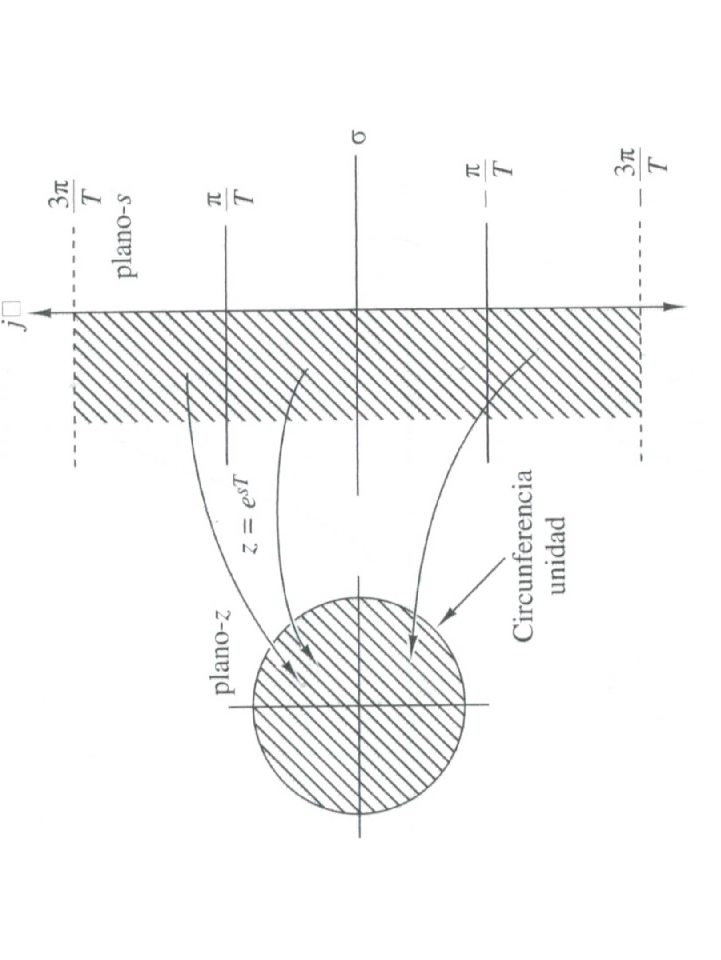
\includegraphics[trim=0cm 1cm 0cm 1cm, clip=true,angle=-90,width=3.5cm]{Figures/Impulso.png}
\end{column}
\end{columns}
}
\visible<4->{
\item \alert{Aproximación por derivadas: $\:\:s= \frac{1-z^{-1}}{T} \: \: \leftrightarrow \:\: z=\frac{1}{1-T\cdot s}$}


\vspace{-0.1cm}
\begin{columns}[c]
\hspace{1cm}\begin{column}{7cm}
\begin{itemize}
\scriptsize
\item Se obtiene sustituyendo la $df(t)/dt$ por $[f(nT)-f((n-1)T)]/T$
\item Puntos del semiplano izquierdo s se relacionan con los puntos internos de la circunferencia pequeña. Se mantiene la estabilidad.
\item Los polos del filtro digital están confinados en la circunferencia pequeña: no se puede diseñar cualquier filtro digital.
\end{itemize}
\end{column}
\hspace{-0.5cm}\begin{column}{3.5cm}
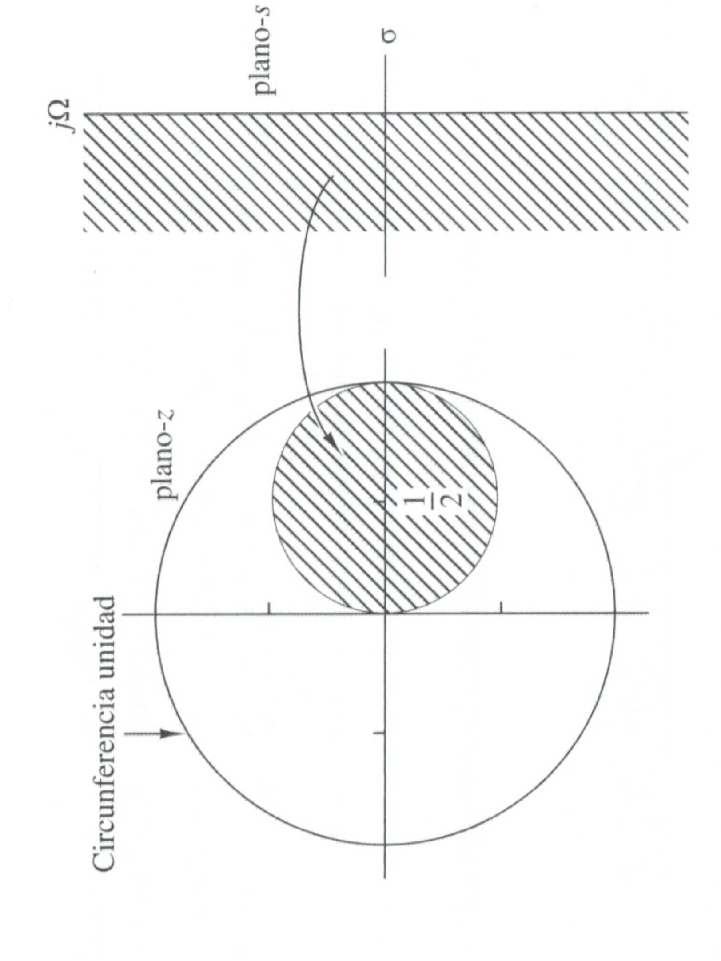
\includegraphics[angle=-90,width=3.5cm]{Figures/Derivada.png}
\end{column}
\end{columns}}
\end{itemize}
\end{itemize}

\end{frame}




%%%%%%%%%%%%%%%%%%%%%%%

\begin{frame}
\frametitle{Transformación del espacio de trabajo ($s \leftrightarrow z$)}
\footnotesize

\begin{itemize}
\item \alert{Filtro continuo $H_a(s)$ $\rightarrow$  filtro discreto: $H(z)=H_a(s)|_{s=F(z)}$}
\item \alert{Transformada bilineal: $\:\:s=\frac{2}{T}\left ( \frac{1-z^{-1}}{1+z^{-1}}\right) \: \: \leftrightarrow \:\: z=\frac{1+T\cdot s/2}{1-T\cdot s/2}$}
\vspace{-0.2cm}
\begin{columns}[T]
\hspace{1cm}\begin{column}{7.5cm}
\begin{itemize}
\scriptsize
\item Se obtiene mediante la aplicación del método de integración numérica trapezoidal a la representación de la ecuación diferencial correspondiente a $H_a(s)$. T es el periodo del paso de integración.

\item Puntos del semiplano izquierdo s se relacionan con los puntos internos a la circunferencia.

\end{itemize}
\end{column}
\begin{column}{4cm}
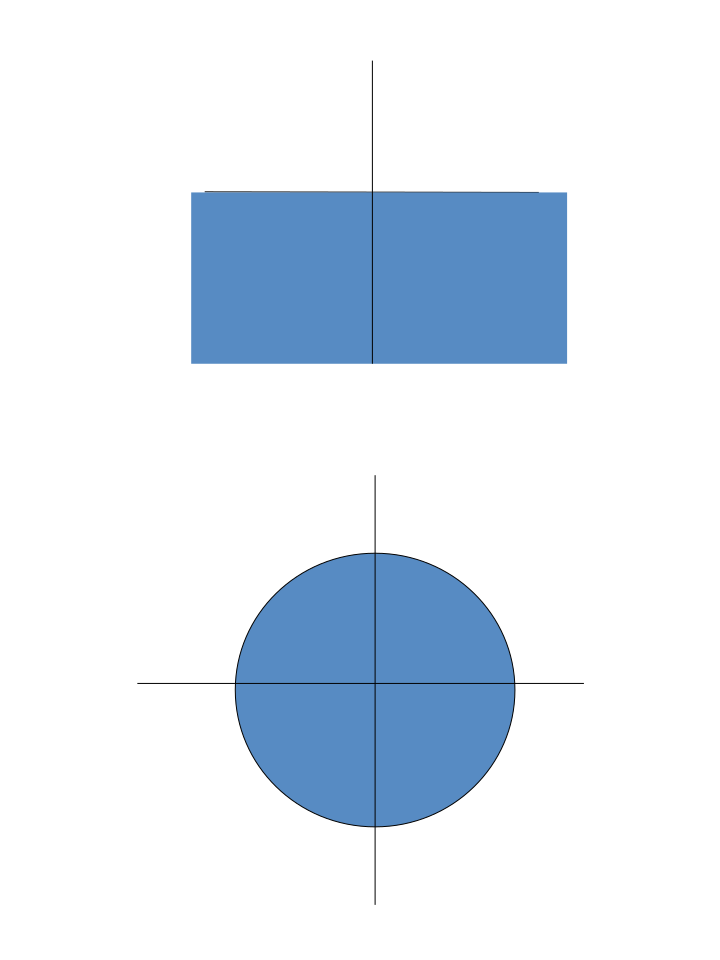
\includegraphics[trim=0cm 0cm 0cm 0cm, clip=true,angle=-90,width=3.5cm]{Figures/Bilineal.png}
\end{column}
\end{columns}


\begin{columns}[T]
\hspace{0.4cm}\begin{column}{11cm}
\begin{itemize}
\scriptsize
\item Es una transformada punto a punto. Se puede utilizar para todos los filtros.

\visible<2->{

\item Relación en frecuencias: \alert{$w_a=\frac{2}{T}tan(w_d/2)$} permite obtener la caracterización del filtro continuo a partir de la caracterización discreta.

\color{gray}
Se establece la relación de s y z con las frecuencias continuas ($s=jw_a$) y discretas ($z=e^{jw_d}$)

$jw_a=\frac{2}{T}\left ( \frac{1-e^{-jw_d}}{1+e^{-jw_d}}\right)=\frac{2}{T}\left ( \frac{e^{jw_d/2}-e^{-jw_d/2}}{e^{jw_d/2}+e^{-jw_d/2}}\right)=\frac{2}{T} j \frac{sen(w_d/2)}{cos(w_d/2)}=\frac{2j}{T} tan(w_d/2)$

Se cumple que  $w_d \!\in \![0,\pi] \leftrightarrow w_a \!\in\! [0,\infty)$; $w_d  \!\in\! [0,-\pi] \leftrightarrow w_a \!\in\! [0,-\infty)$
}
\visible<3->{
\color{black}
\item Se produce un combado de las frecuencias, asociado al comportamiento no lineal de la tangente.
}
\visible<4->{
\item \alert{Si hacemos T=2, las expresiones se simplifican.}
}
\end{itemize}
\end{column}
\end{columns}

\end{itemize}

\end{frame}



%%%%%%%%%%%%%%%%%%%%%%%

\begin{frame}
\frametitle{Diseño de filtros IIR paso bajo}
\small
\begin{enumerate}
\item Aplicar la relación entre las frecuencias ($w_a=\frac{2}{T}tan(w_d/2)$) para obtener la especificación en frecuencias del filtro continuo.
\item Diseñar el filtro continuo correspondiente (Butterworth, Chebyshev, Elíptico). Obtener su función de transferencia $H_a(s)$.
\item Aplicar la transformada bilineal ($s=\frac{2}{T}\left ( \frac{1-z^{-1}}{1+z^{-1}}\right)$) para obtener la función de transferencia del filtro discreto.
\begin{itemize}
\item Con Matlab: \alert{\texttt{[numz,denz]=bilinear(nums,dens,1/T)}}
\end{itemize}

\item Representar la respuesta en frecuencia del filtro (no hay que normalizarlo).
\begin{itemize}
\item Con Matlab: \alert{\texttt{[Hw,w]=freqz(numz,denz)}}


\end{itemize}

\end{enumerate}

\rule{12cm}{0.4pt}
\footnotesize

T=2 para simplificar las expresiones, hacen de la orden bilineal se llamen con tercer parámetro igual a 0.5.

\end{frame}

%%%%%%%%%%%%%%%%%%%%%%%%%%



\begin{frame}
\frametitle{Ejemplo de diseño de filtro  IIR paso bajo}

\footnotesize
\color{olivegreen} Diseñar un IIR de Butterworth paso bajas que opera con una tasa de muestreo de 200 KHz, con una frecuencia de paso de 25KHz y una frecuencia supresora de 55KHz, con un rizo paso banda que no exceda los 0.5 dB y una atenuación mínima en la banda supresora de 15dB.
\color{gray}
\vspace{0.1cm}

1)  Especificaciones del filtro continuo:

\vspace{0.1cm}

$\left . \begin{array}{l}w_{pd}=w_pT_s=2\pi 25/200=0.25\pi\\w_{sd}=w_sT_s=2\pi 55/200=0.55\pi\end{array}\right \}$ $\rightarrow \left . \begin{array}{l}w_{pa}=tan(w_{pd}/2)=0.4142\\w_{sa}=tan(w_{sd}/2)=1.1708\end{array}\right \}$

\vspace{0.1cm}

2) Cálculo del filtro continuo (utilizando expresiones/Matlab):

\vspace{0.1cm}

\hspace{0.3cm}\texttt{[N,wca]=buttord(0.4142,1.1708,.5,15,'s')}

\vspace{0.1cm}

\hspace{0.3cm}\texttt{[numc,denc]=butter(N,wca,'low','s')};

\vspace{0.1cm}

\begin{columns}[T]
\begin{column}{7cm}
3) Conversión al filtro discreto

\vspace{0.1cm}

\hspace{0.3cm}\texttt{[numd,dend]=bilinear(numc,denc,0.5)}

\vspace{0.1cm}

4) Representación del espectro del filtro:

\vspace{0.1cm}

\hspace{0.3cm}\texttt{[Hw,w]=freqz(numz,denz)}

\vspace{0.1cm}

\hspace{0.3cm}\texttt{plot(w/pi,abs(Hw))}
\end{column}
\begin{column}{4cm}

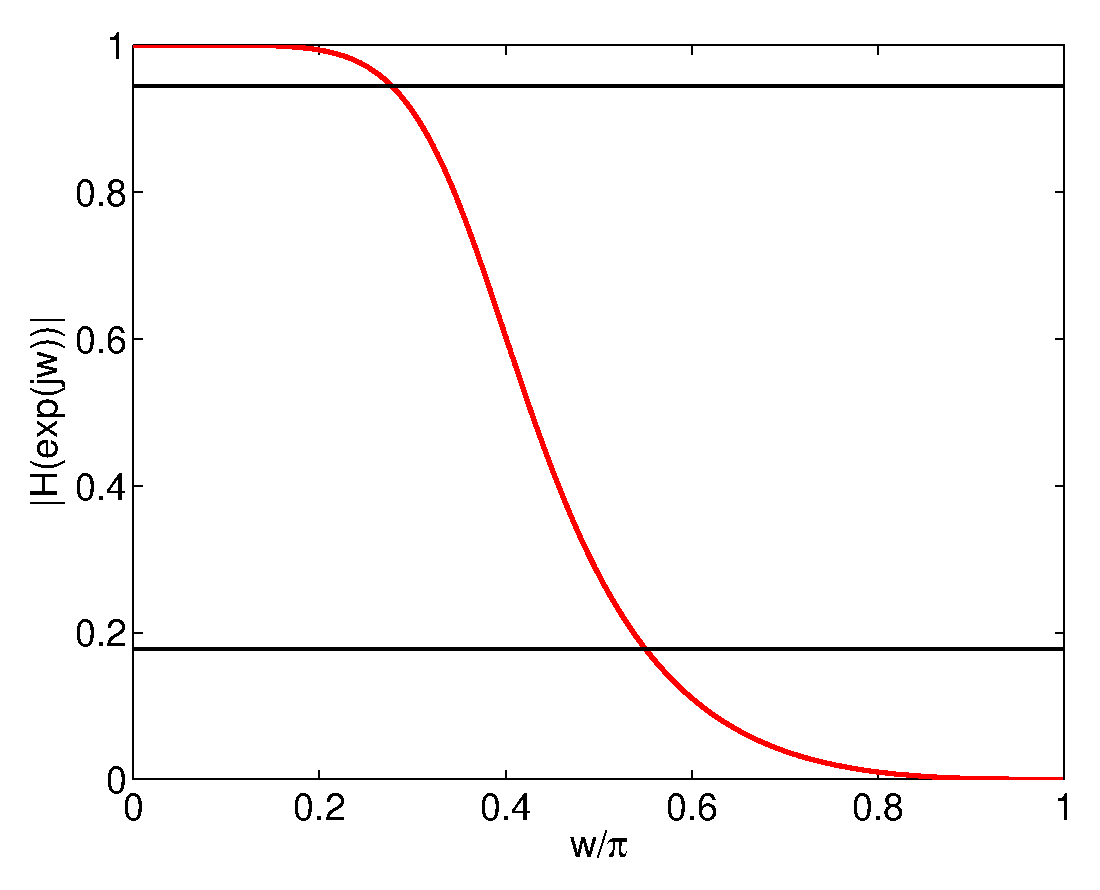
\includegraphics[width=4cm]{Figures/FiltroDiscretoPB_Butter.eps}
\end{column}
\end{columns}


\end{frame}

%%%%%%%%%%%%%%%%%%%%%%%%%%%%


\begin{frame}
\frametitle{Filtros  IIR paso alto, paso banda, supresor de banda}
\small

\visible<2->{
\vspace{-0.4cm}
\begin{enumerate}
\item Aplicar la relación entre las frecuencias ($w_a=\frac{2}{T}tan(w_d/2)$) para obtener la especificación en frecuencias del filtro continuo $H_a(s)$.
\vspace{-0.1cm}
\item Convertir las especificaciones del filtro continuo $H_a(s)$ en las de un filtro paso baja continuo $H_{LP}(s)$.
\vspace{0.1cm}

\begin{columns}[T]
\hspace{0.8cm}\begin{column}{2cm}
\scriptsize
Paso alto:

\vspace{0.2cm}

$s=\frac{w_p \hat w_p}{\hat s}$

\vspace{0.2cm}

 $- w \hat w=w_p \hat w_p$
\end{column}
\hspace{-0.8cm}\begin{column}{3cm}
\scriptsize
Paso banda:

\vspace{0.1cm}

 $s=w_p\frac{\hat s^2+\hat w_0^2}{\hat s (\hat w_{p2}-\hat w_{p1})}$

$w=w_p\frac{\hat w^2-\hat w_0^2}{\hat w (\hat w_{p2}-\hat w_{p1})}$

$\hat w_0^2=\hat w_{p1}\hat w_{p2}=\hat w_{s1}\hat w_{s2}$

\end{column}
\hspace{-0.8cm}\begin{column}{3cm}
\scriptsize
Supresor de banda:

\vspace{0.1cm}

$s=w_s\frac{\hat s (\hat w_{s2}-\hat w_{s1})}{\hat s^2+\hat w_0^2}$

$w=w_s\frac{\hat w (\hat w_{s2}-\hat w_{s1})}{\hat w_0^2-\hat w^2}$

$\hat w_0^2=\hat w_{p1}\hat w_{p2}=\hat w_{s1}\hat w_{s2}$


\end{column}

\end{columns}

\vspace{-0.2cm}

\item Diseñar el filtro continuo paso bajas $H_{LP}(s)$

\vspace{-0.1cm}
}
\visible<4->{
\item Seguir uno de los dos procedimientos siguientes:
}
\end{enumerate}
\vspace{-0.3cm}
\begin{columns}[T]
\begin{column}{5.5cm}
\footnotesize \visible<5->{
\hspace{1.5cm}Procedimiento 1
\begin{itemize}
\scriptsize
\item Convertir el filtro paso baja $H_{LP}(s)$ en el filtro destino $H_a(s)$ usando la relación espectral correspondiente.
\vspace{-0.1cm}
\item  Convertir el filtro $H_a(s)$ en el filtro discreto $H(z)$ con la transformación bilineal ($s=\frac{2}{T}\left ( \frac{1-z^{-1}}{1+z^{-1}}\right)$)
\end{itemize}}
\end{column}
\begin{column}{5.5cm}
\footnotesize \visible<6->{
\hspace{1.5cm}Procedimiento 2
\begin{itemize}
\scriptsize
\item Convertir el filtro paso baja $H_{LP}(s)$ en el filtro $H_{LP}(z)$ con la  transformación bilineal ($s=\frac{2}{T}\left ( \frac{1-z^{-1}}{1+z^{-1}}\right)$).
\vspace{-0.1cm}
\item Convertir el filtro $H_{LP}(z)$ en el filtro destino $H(z)$ usando la relación espectral discreta correspondiente.
\end{itemize}}
\end{column}
\end{columns}
\end{frame}



\begin{frame}
\frametitle{Ejemplo de un filtro  IIR  paso alto}
\footnotesize

\footnotesize
\color{olivegreen} Diseñar con el procedimiento 1 un IIR de Chebyshev Tipo 1 paso altas con las siguientes características: borde de la frecuencia de paso 700Hz, borde de la banda supresora 500Hz, rizo paso banda 1dB, atenuación mínima banda supresora 32 dB, frecuencia de muestreo 2KHz.
\color{gray}
\vspace{0.1cm}

1)  Obtener las especificaciones del filtro continuo paso alta $H_a(s)$:

$\left . \begin{array}{l}w_{pd}=w_pT_s=2\pi 700/2000=0.7\pi\\w_{sd}=w_sT_s=2\pi 500/2000=0.5\pi\end{array}\right \}$ $\rightarrow \left . \begin{array}{l}\hat w_{pa}=tan(w_{pd}/2)=1.9626\\\hat w_{sa}=tan(w_{sd}/2)=1.0\end{array}\right \}$

\vspace{0.1cm}

2) Obtener las especificaciones del filtro continuo paso baja $H_{LP}(s)$:

\vspace{0.1cm}


\hspace{0.25cm}$w\hat w=w_{pa}\hat w_{pa}$. Suponiendo que $w_{pa}=1 \rightarrow w_{sa}=\hat w_{pa}/\hat w_{sa}=1.9626$.

\vspace{0.1cm}

\begin{columns}[T]
 \hspace{0.2cm}\begin{column}{7.7cm}
3) Diseño filtro Chebyshev Tipo 1

\vspace{0.1cm}

\hspace{0.25cm}\texttt{[N,wn]=cheb1ord(1,1.9626,1,32,'s')}

\hspace{0.25cm}\texttt{[numlp,denlp]=cheby1(N,1,wn,'low','s')}

\vspace{0.1cm}

 4) Seguir el procedimiento 1:

 \vspace{0.1cm}

 \hspace{0.25cm}\texttt{[numhp,denhp]=lp2hp(numlp,denlp,1.9626)}

\hspace{0.25cm}\texttt{[numz,denz]=bilinear(numhp,denhp,0.5);}
 \end{column}
 \hspace{-0.5cm}\begin{column}{3.8cm}
 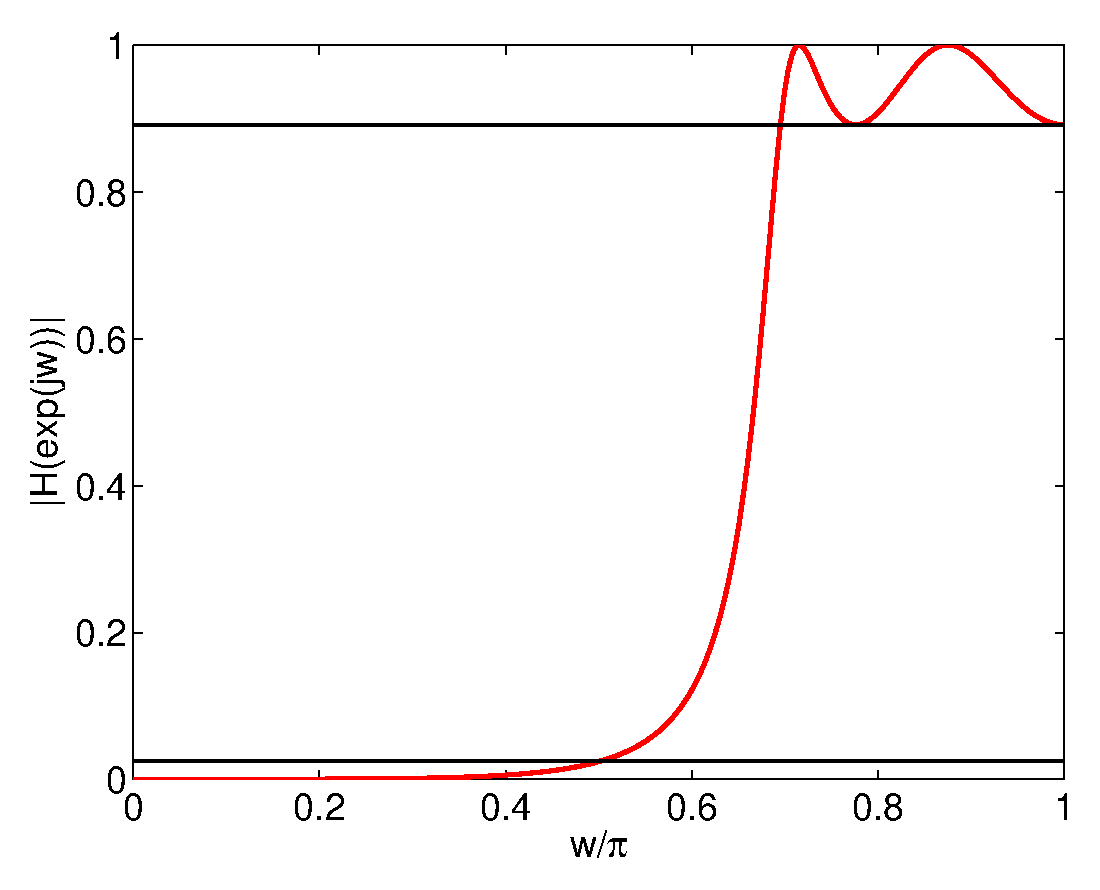
\includegraphics[width=3.8cm]{Figures/FiltroDiscretoPA_Cheby1.eps}
 \end{column}
 \end{columns}

\end{frame}


%%%%%%%%%%%%%%%%%%%%%%%%%%%%%%%%



\begin{frame}
\frametitle{Ejemplo de un filtro  IIR paso banda}
\footnotesize

\footnotesize
\color{olivegreen} Diseñar con el procedimiento 1 un IIR de Butterworth paso banda con las siguientes características: bordes normalizados de la banda de paso 0.45$\pi$ y 0.65$\pi$, bordes normalizados de la banda supresora 0.3$\pi$ y 0.75$\pi$, rizo paso banda 1dB, atenuación mínima banda supresora 40 dB.
\color{gray}
\vspace{0.1cm}

1)  Características del filtro continuo paso banda $H_a(s)$, usando $\hat w_{a}=tan(w_{d}/2)$  :

$\begin{array}{ll}w_{p1d}=0.45\pi \rightarrow \hat w_{p1a}=0.8541 &\:\: w_{p2d}=0.65\pi \rightarrow \hat w_{p2a}=1.6319 \\
w_{s1d}=0.3\pi \rightarrow \hat w_{s1a}=0.5095 &\:\: w_{s2d}=0.75\pi \rightarrow \hat w_{s2a}=2.4142
\end{array}$

\vspace{0.1cm}

2) Obtener las especificaciones del filtro continuo paso baja $H_{LP}(s)$:

\vspace{0.1cm}

$\left . \begin{array}{l}\hat w_0^2 =\hat w_{p1a}\hat w_{p2a}=1.3938\\w_0^2 =\hat w_{s1a}\hat w_{s2a}=1.23
\end{array} \right \}$ $\rightarrow \hat w_{s1a}=\frac{1.3938}{w_{s2a}}=0.5772$, $\hat w_0=1.1806$


\hspace{0.25cm}Si $w_p=1$, $w_{s}=w_p\frac{\hat w_{s1a}^2-\hat w_0^2}{\hat w_{s1a} (\hat w_{p2}-\hat w_{p1})}=2.3617$


\vspace{0.1cm}

\begin{columns}[T]
 \hspace{0.2cm}\begin{column}{7.7cm}
3) Diseño filtro Butterworth

\vspace{0.1cm}

\hspace{0.25cm}\texttt{[N,wn]=buttord(1,2.3617,1,40,'s')}

\hspace{0.25cm}\texttt{[nlp,dlp]=butter(N,wn,'low','s')}

\vspace{0.1cm}

 4) Seguir el procedimiento 1:

 \vspace{0.1cm}
  \hspace{0.28cm}\texttt{banda=1.6139-0.8541;}

 \hspace{0.25cm}\texttt{[npb,dpb]=lp2bp(nlp,dlp,1.1806,banda)}

\hspace{0.25cm}\texttt{[numz,denz]=bilinear(npd,dpd,0.5);}
 \end{column}
 \hspace{-0.5cm}\begin{column}{3.8cm}
 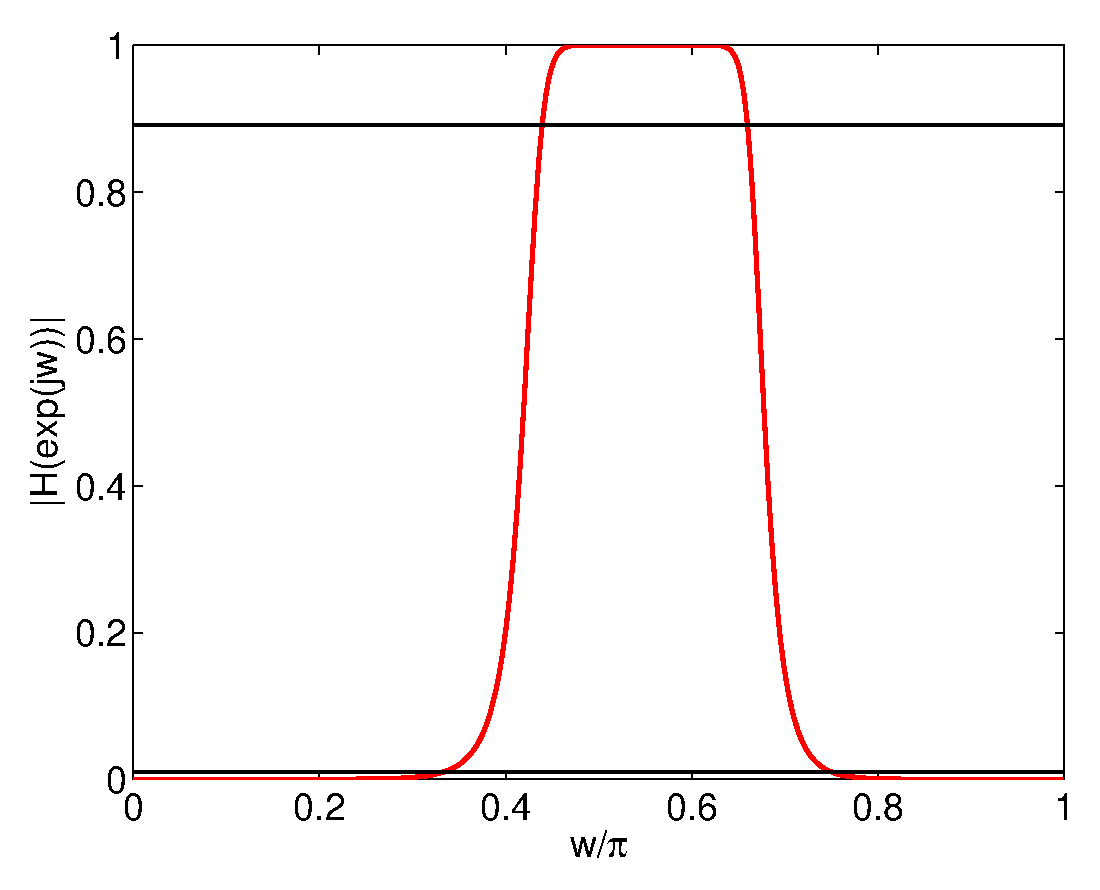
\includegraphics[width=3.8cm]{Figures/FiltroDiscretoPBanda_Butter.eps}
 \end{column}
 \end{columns}

\end{frame}

%%%%%%%%%%%%%%%%%%%%%%%%%%%%%%%%%%%%%%%%%%%%%%%%%%%%%

\begin{frame}
\frametitle{Relaciones espectrales discretas}

\begin{itemize}
\footnotesize
\item La transformación espectral discreta $z=F(\hat z)$ permite obtener a partir de un filtro discreto paso bajo $H_{LP}(z)$  otro filtro discreto$^1$ (paso alto, paso banda, supresor de banda) $H(\hat z)=H_{LP}(z)|_{z=F(\hat z)}$.
\begin{itemize}
\footnotesize

\item Filtro paso alta: $z^{-1}=-\frac{\hat z^{-1}+\lambda}{1+\lambda \hat z^{-1}}$, con
$\lambda=-\frac{cos((w_c-	\hat w_c)/2)}{cos((w_c+	\hat w_c)/2)}$



\item Filtro paso banda: $z^{-1}=-\frac{\hat z^{-2}-\frac{2\lambda \rho}{\rho+1}\hat z^{-1}+\frac{\rho-1}{\rho+1}}{\frac{\rho-1}{\rho+1}\hat z^{-2}-\frac{2\lambda \rho}{\rho+1}\hat z^{-1}+1}$,

$\lambda=\frac{cos((\hat w_{c2}+	\hat w_{c1})/2)}{cos((\hat w_{c2}-	\hat w_{c1})/2)}$, $\rho=\cot((\hat w_{c2}-\hat w_{c1})/2)\tan(w_c/2)$

\item Filtro supresor banda: $z^{-1}=\frac{\hat z^{-2}-\frac{2\lambda}{\rho+1}\hat z^{-1}+\frac{1-\rho}{\rho+1}}{\frac{1-\rho}{\rho+1}\hat z^{-2}-\frac{2\lambda}{\rho+1}\hat z^{-1}+1}$,

$\lambda=\frac{cos((\hat w_{c2}+\hat w_{c1})/2)}{cos((\hat w_{c2}-\hat w_{c1})/2)}$, $\rho=\tan((\hat w_{c2}-\hat w_{c2})/2)\tan(w_c/2)$


\end{itemize}

\item Con Matlab$^{2}$
\begin{itemize}
\footnotesize
\item \texttt{[npa,dpa]=iirlp2hp(numlp,denlp,wplp,wphp)}
\item \texttt{[npa,dpa]=iirlp2bp(numlp,denlp,wplp,[wp1d,wp2d])}
\item \texttt{[nbs,dbs]=iirlp2sp(numlp,denlp,wslp,[ws1d,ws2d])}
\end{itemize}
\end{itemize}

\vspace{-0.2cm}
\rule{10cm}{0.4pt}

\scriptsize
$^1$También existe una relación espectral que permite transformar un filtro paso bajo en otro paso bajo, que se utiliza para cambiar las especificaciones en frecuencia de un filtro paso baja ya diseñado.

$^2$ Las frecuencias tienen que estar  normalizadas entre $[0,1]$ que se corresponden a los valores discretos entre $[0,\pi]$


\end{frame}



\begin{frame}
\frametitle{Ejemplo de un filtro  IIR paso banda}
\footnotesize

\footnotesize
\color{olivegreen} Diseñar con el procedimiento 2 un IIR de Butterworth paso banda con las siguientes características: bordes normalizados de la banda de paso 0.45$\pi$ y 0.65$\pi$, bordes normalizados de la banda supresora 0.3$\pi$ y 0.75$\pi$, rizo paso banda 1dB, atenuación mínima banda supresora 40 dB.
\color{gray}
\vspace{0.1cm}

1)  Características del filtro continuo paso banda $H_a(s)$, usando $\hat w_{a}=tan(w_{d}/2)$  :

$\begin{array}{llll}\hat w_{p1a}=0.8541 &\hat w_{p2a}=1.6319  & \hat w_{s1a}=0.5095 & \hat w_{s2a}=2.4142
\end{array}$

\vspace{0.1cm}

2) Obtener las especificaciones del filtro continuo paso baja $H_{LP}(s)$:

\vspace{0.1cm}

\hspace{0.25cm}$\hat w_{s1a}=\frac{1.3938}{w_{s2a}}=0.5772$, $\hat w_0=1.1806$, $w_p=1$, $w_{s}=2.3617$


\vspace{0.1cm}

\begin{columns}[T]
 \hspace{0.2cm}\begin{column}{7.7cm}
3) Diseño filtro Butterworth

\vspace{0.1cm}

\hspace{0.25cm}\texttt{[N,wn]=buttord(1,2.3617,1,40,'s')}

\hspace{0.25cm}\texttt{[nlp,dlp]=butter(N,wn,'low','s')}

\vspace{0.1cm}

 4) Seguir el procedimiento 2:

 \vspace{0.1cm}

  \hspace{0.25cm}\texttt{[nlpz,dlpz]=bilinear(nlp,dlp,0.5);}

\visible<2->{
  \hspace{0.25cm}\texttt{[Hlpw,w]=freqz(nlpz,dlpz);}

  \hspace{0.25cm}\texttt{plot(w/pi,abs(Hw))}

   \hspace{0.25cm}\texttt{plot(w/pi,10\^ (-1/20)*ones(length(w),1))};

  }

 \visible<3->{
  \hspace{0.25cm}\texttt{a=ginput(1);} \hspace{0.25cm}\texttt{wp=a(1);}}

  \hspace{0.25cm}\texttt{wpasod=[0.45,0.65];}


 \hspace{0.25cm}\texttt{[nz,dz]=irrlp2bp(nlpz,dlpz,wp,wpasod)}


 \end{column}
 \hspace{-0.5cm}\begin{column}{3.8cm}
\only<2-3|handout=0>{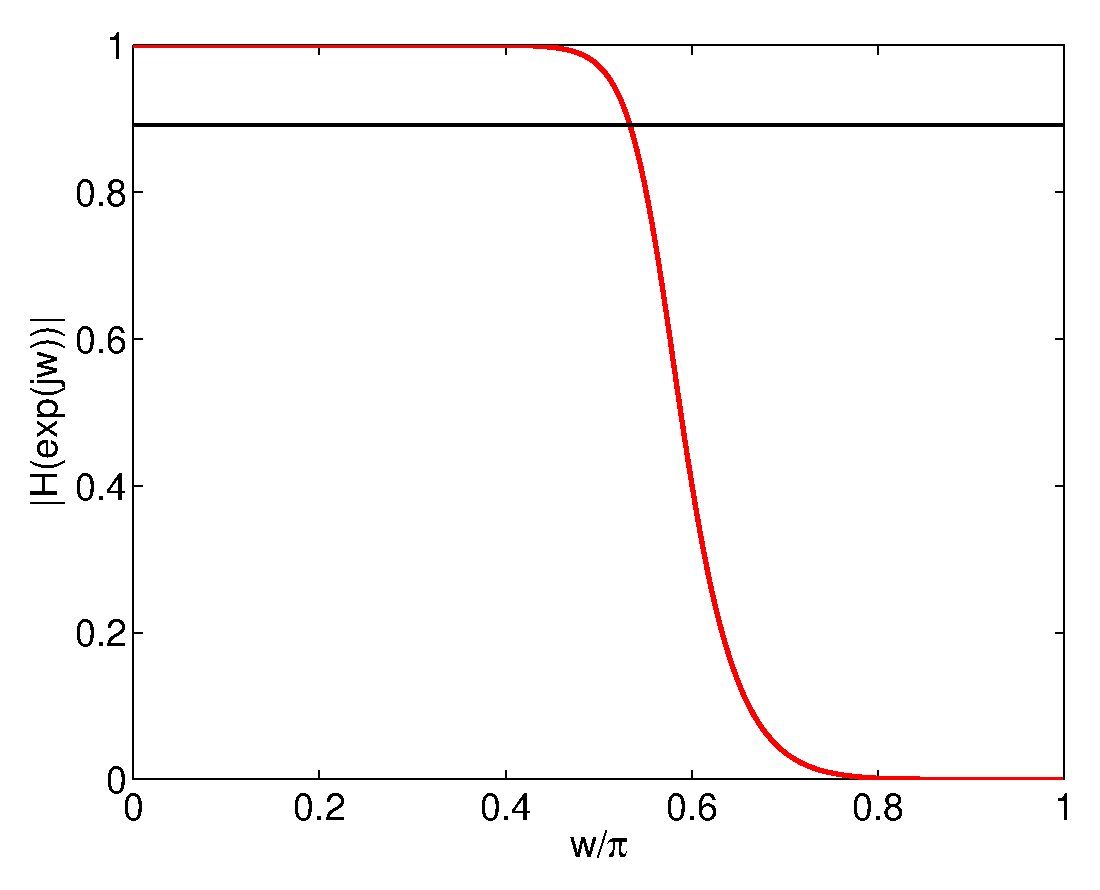
\includegraphics[width=3.8cm]{Figures/FiltroDiscretoPBanda_Butter21.eps}}
\visible<4->{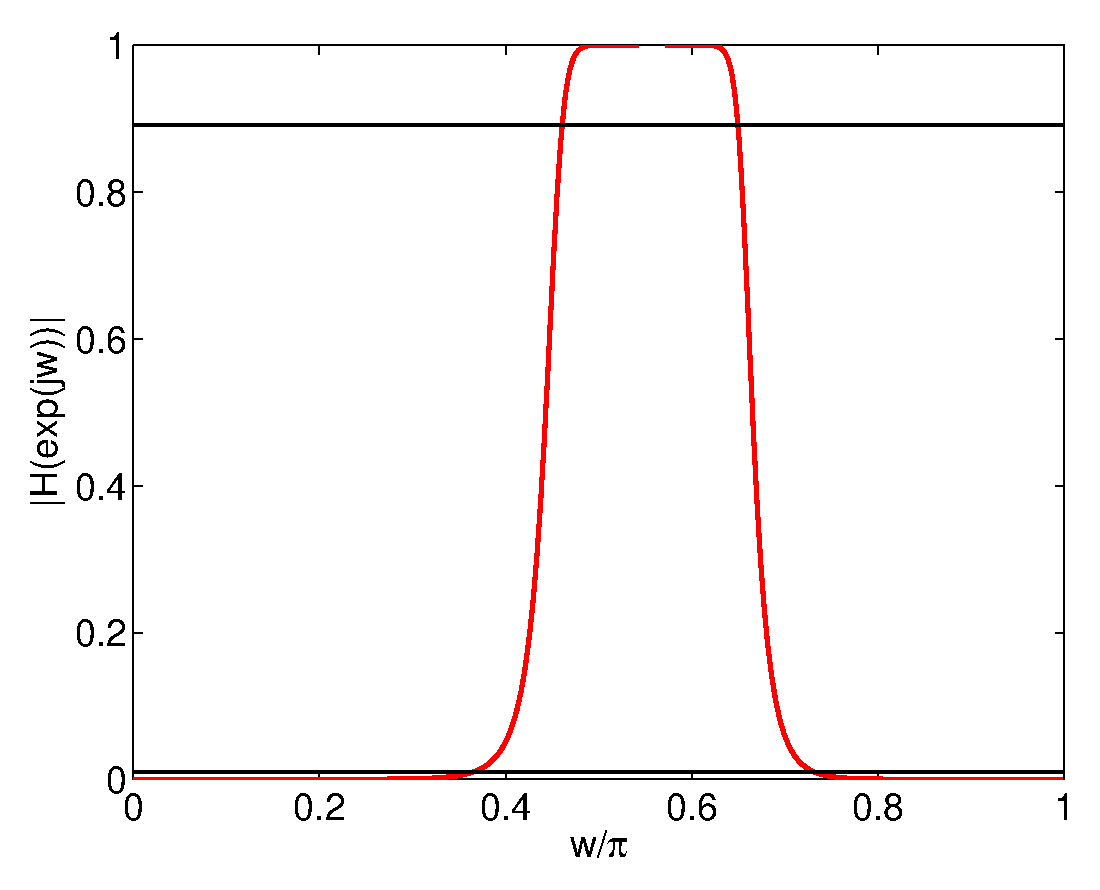
\includegraphics[width=3.8cm]{Figures/FiltroDiscretoPBanda_Butter22.eps}}

 \end{column}
 \end{columns}

\end{frame}

%%%%%%%%%%%%%%%%%%%%%%%%%%%%%%%%%%%%%%%%


\begin{frame}
\frametitle{Diseño de filtros  IIR con Matlab}
\footnotesize
\begin{itemize}
\item Matlab permite realizar directamente el diseño de los filtros discretos, sin necesidad de realizar los pasos intermedios.
\item Para ello, hay que poner en las funciones que ya conocemos las frecuencias normalizadas [0,1] y eliminar la llamada a 's'.

\item Veamos un ejemplo con las funciones de Chebyshev de tipo II
\begin{itemize}
\item \alert{\texttt{[N,wn]=cheb2ord(wp,ws,alphap,alphas);}}

\vspace{0.1cm}

{\footnotesize
\hspace{0.5cm}Paso bajo: wp=0.3, ws=0.5;

\vspace{0.1cm}

\hspace{0.5cm}Paso alto: wp=0.5, ws=0.3;

\vspace{0.1cm}

\hspace{0.5cm}Paso banda: wp=[0.5 0.7], ws=[0.4 0.8];

\vspace{0.1cm}

\hspace{0.5cm}Eliminación de banda: wp=[0.5 0.7], ws=[0.55 0.65];}

\vspace{0.1cm}

\item\alert{\texttt{[num,den]=cheby2(N,alphas,wn,tipo);}}

\vspace{0.1cm}

\hspace{0.5cm}tipo: 'low', 'high', nada, 'stop'

\end{itemize}


\item Los resultados de Matlab coinciden con los obtenidos a través del procedimiento 1.

\end{itemize}

\end{frame}





\begin{frame}
\frametitle{Ejemplo de un filtro  IIR paso banda}
\footnotesize

\footnotesize
\color{olivegreen} Diseñar directamente con Matlab un IIR de Butterworth paso banda con las siguientes características: bordes normalizados de la banda de paso 0.45$\pi$ y 0.65$\pi$, bordes normalizados de la banda supresora 0.3$\pi$ y 0.75$\pi$, rizo paso banda 1dB, atenuación mínima banda supresora 40 dB.
\color{gray}
\vspace{0.1cm}


\vspace{0.1cm}

\begin{columns}[T]
\begin{column}{6cm}
\lstinputlisting{./Matlab/ButterDCode.m}


 \end{column}
\hspace{-0.5cm} \begin{column}{4.5cm}
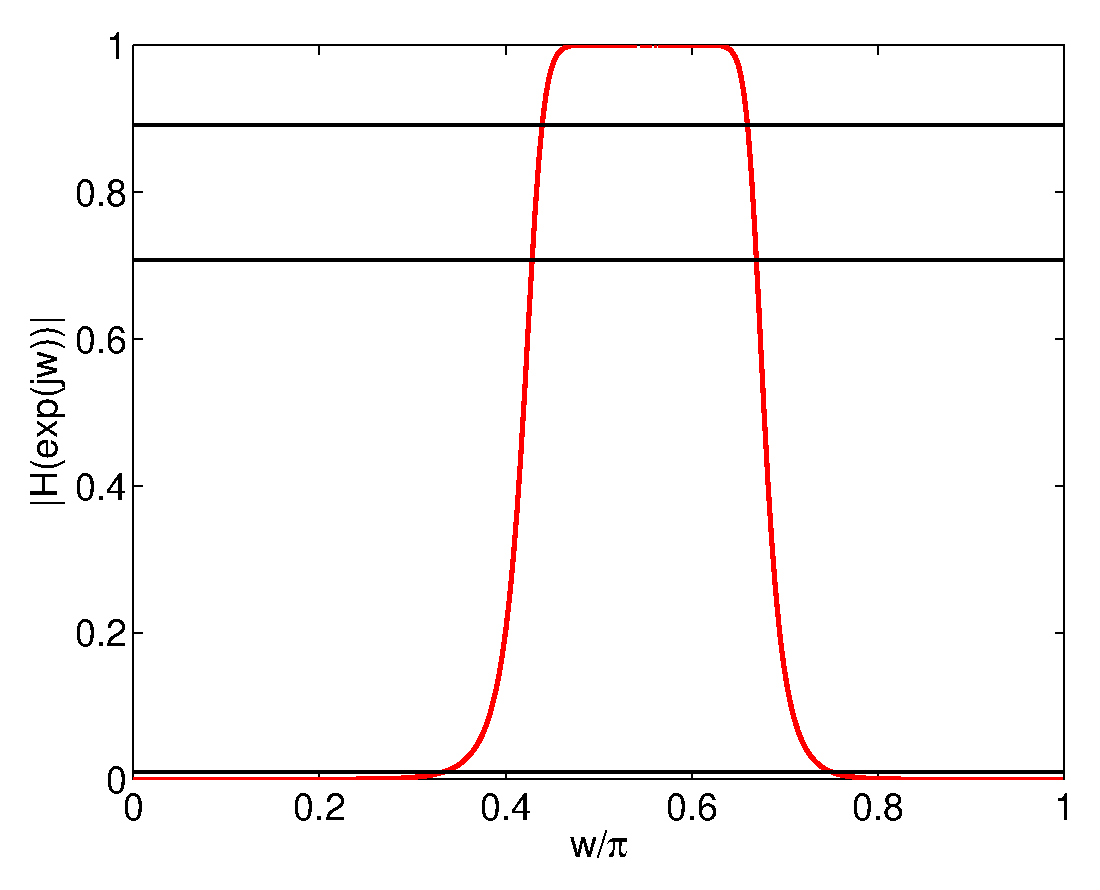
\includegraphics[width=4.5cm]{Figures/FiltroDiscretoPBanda_ButterMatlab.eps}

 \end{column}
 \end{columns}

\end{frame}


\subsection{Filtros FIR}

\begin{frame}
\frametitle{Procedimiento de diseño de filtros FIR}

\begin{itemize}
\footnotesize
\item Los filtros discretos FIR no tienen conexión directa con ningún filtro continuo, y por lo tanto, su diseño no se puede basar en la construcción de ningún filtro analógico.

\visible<2->{\item El diseño de estos filtros se basa en la aproximación directa de la respuesta en frecuencia deseada (i.e. calcular los valores de $h(n)$ para que $H(e^{jw})$ tenga la forma deseada).

\hspace{0.8cm}$H(e^{jw})=\sum_{n=-\infty}^{\infty} h(n)e^{-jwn} \rightarrow H(e^{jw})=\sum_{n=0}^{N} h(n)e^{-jwn} $   }

\visible<3->{
\item Los filtros que vamos a estudiar cumplen dos propiedades adicionales: son filtros con \alert{$h(n)$ real} y \alert{fase lineal} en la respuesta en frecuencia: $arg(H(e^{jw}))=\alpha w+\beta$. Ambos hechos\visible<5->{$^1$} hacen que el desfase sea introducido por el filtro a cada frecuencia sea $-Nw/2$.

\begin{itemize}
\footnotesize
\item Transformada de Fourier con ventana.
\item \color{gray} Muestreo en frecuencia.\color{black}
\item Diseño asistido por computador.
\end{itemize}
}

\visible<4->{
\item Veremos que para diseñar los filtros será necesario primero estimar el valor $N$ y a continuación los valores de las h(n).
}

\end{itemize}

\visible<5->{
\rule{12cm}{0.4pt}
\scriptsize
$^1$ Al final del tema veremos las propiedades que cumplen todos los filtros FIR con $h(n)$ real y fase lineal. En esta sección nos centraremos en el diseño de un subconjunto de estos filtros.}
\end{frame}



\begin{frame}
\frametitle{Diseño FIR por la TF con ventana  }

\vspace{-0.2cm}

\footnotesize


\begin{itemize}
\item La TF en tiempo discreto relaciona la respuesta en frecuencia del filtro con la respuesta del filtro a la señal impulso $h(n)$.  La segunda expresión permite obtener la $h_d(n)$ a partir de la respuesta en frecuencia $H_d(e^{jw})$.



\hspace{1cm}$H_d(e^{jw})=\sum_{n=-\infty}^{\infty}h_d(n)e^{-jwn}$

\hspace{1cm}$h_d(n)=\frac{1}{2\pi}\int_{-\pi}^\pi H_d(e^{jw}) e^{jwn} dw\:\:$  con $\:\:\infty \le n \le \infty$


\end{itemize}

\vspace{-0.3cm}

\visible<2->{

\begin{columns}[c]
\begin{column}{8cm}
\begin{itemize}

\item El problema surge cuando se desea diseñar un filtro cuya respuesta en frecuencia toma un valor constante en módulo por secciones, ya que esto implica que la respuesta a la función impulso es de longitud doblemente infinita (no causal y distinta de cero $\:\:\infty \le n \le \infty$).
\end{itemize}
\end{column}
\hspace{-0.4cm}\begin{column}{3cm}
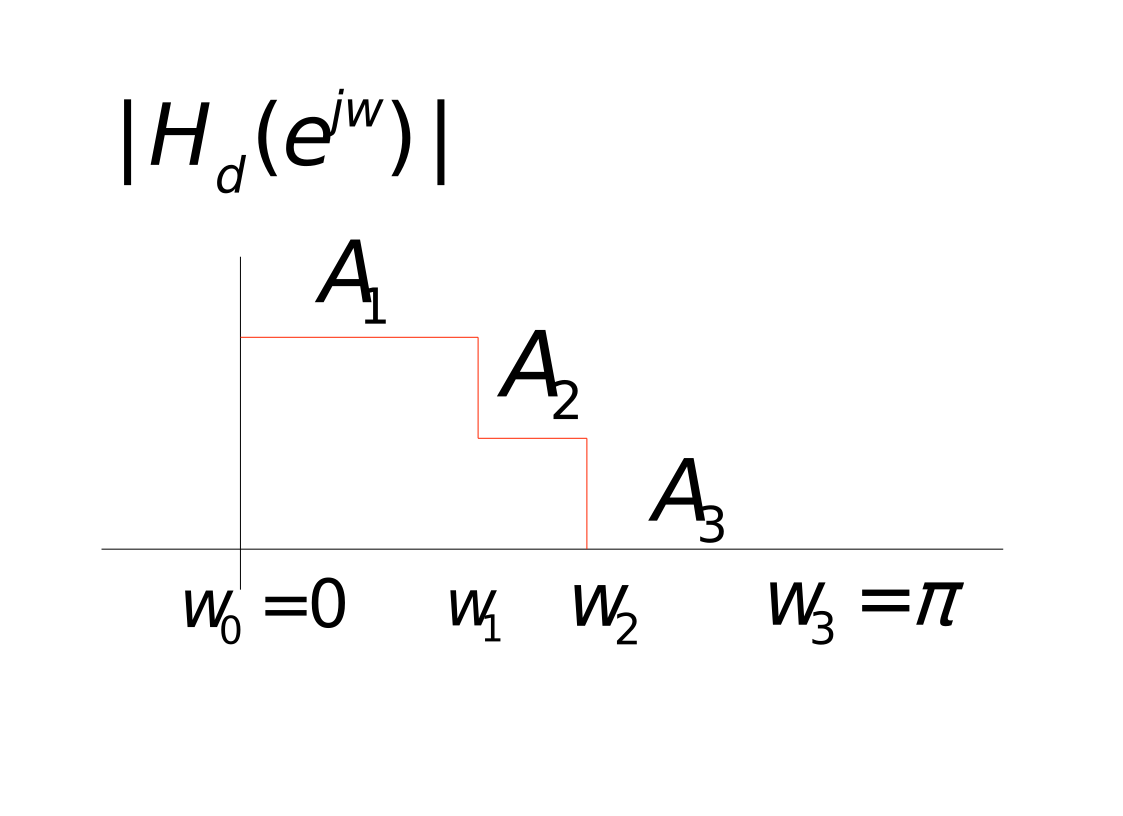
\includegraphics[trim=0cm 1cm 0cm 1cm,clip=true,width=3.5cm]{Figures/PorTramos}
\end{column}
\end{columns}
}

\vspace{-0.1cm}
\begin{itemize}

\visible<3->{
\item Para convertir el filtro deseado $h_d(n)$ en un FIR de orden N+1 podemos:
}

\begin{enumerate}
\footnotesize
\visible<4->{\item Limitar el tamaño de la respuesta al impulso (truncarla/enventanarla,  $h_t(n)=v(n)h_d(n)$) con una ventana $v(n)$ de tamaño 2L+1=N+1.}
\visible<5->{
\item Retardar la respuesta del filtro $L=N/2$ unidades, para convertirlo en causal: $h(n)=h_t(n-L)$. Esto permite que el desfase en frecuencia sea lineal ya que $H(e^{jw})=e^{-jLw}H_t(e^{jw})=e^{-jwN/2}H_t(e^{jw})$.
}
\end{enumerate}
\end{itemize}

\vspace{-0.2cm}

\visible<6->{
\rule{12cm}{0.4pt}
\scriptsize
$h_d(n)$ es el filtro que $d$eseamos diseñar, $h_t(n)$ el sistema  que se obtiene $t$runcando/enventanando $h_d(n)$, y h(n) el filtro FIR (causal) final. }
\end{frame}

%%%%%%%%%%%%%%%%%%%%%%%%%%

\begin{frame}
\frametitle{Respuesta al impulso de filtros deseados I}
\footnotesize

\begin{itemize}
\item Se calcula la $h_d(n)$  de los filtros deseados con $h_d(n)\!=\!\frac{1}{2\pi}\!\!\int_{-\pi}^\pi H_d(e^{jw}) e^{jwn} dw$ o a través de las propiedades de la TFDT.
\end{itemize}

\begin{columns}[T]


\begin{column}{5cm}
\scriptsize
\visible<2->{\centering{
\alert{Filtro paso bajo}}


\vspace{0.1cm}

$\scriptsize H_{LPd}(e^{jw})\!=\!\left \{  \!\!\!\begin{array}{l} 1, \:\:\: |w|\!\!<\!\!w_c\\0,\:\:\: w_c\le |w| \le \pi \end{array}\right .$


\vspace{0.1cm}
\color{gray}$h_{LPd}(n)=\frac{1}{2\pi}\int_{-w_c}^{w_c} e^{jwn}dw$\color{black}


\vspace{0.1cm}
$h_{LPd}(n)=\!\left \{\!\!\!\begin{array}{l}\frac{w_c}{\pi}, \:\:\:  \:\:\: \:\:\: n=0\\ \frac{sen(nw_c)}{\pi n},  \:\:\: c.c.\end{array}  \right . $


\vspace{0.1cm}
}
\visible<3->{
\scriptsize
\centering{
\alert{Filtro paso alto}}

\vspace{0.1cm}
$\scriptsize H_{HPd}(e^{jw})\!=\!\left \{  \!\!\!\begin{array}{l} 0, \:\:\: |w|\!\!<\!\!w_c\\1,\:\:\: w_c\le |w| \le \pi \end{array}\right .$


\vspace{0.1cm}

\color{gray}
$H_{HPd}(e^{jw})=1-H_{LPd}(e^{jw})$

\vspace{0.1cm}

$h_{HPd}(n)=\delta(n)-h_{LPd}(n)$

\color{black}

\vspace{0.1cm}

$h_{HPd}(n)=\!\left \{\!\!\!\begin{array}{l}1-\frac{w_c}{\pi}, \:\:\:  \:\:\: \:\:\: n=0\\ -\frac{sen(nw_c)}{\pi n},  \:\:\: c.c.\end{array}  \right . $

}

\end{column}
\begin{column}{5.5 cm}
\scriptsize
\visible<4->{
\centering{
\alert{Filtro paso banda}}

\vspace{0.1cm}


$\scriptsize H_{BPd}(e^{jw})\!=\!\left \{  \!\!\!\begin{array}{l} 1, \:  w_{1}\!\!<\!\!|w|\!\!<\!\!w_{2}\\0, \:\textrm{c.c.}  \end{array}\right .$


\vspace{0.1cm}
\color{gray}


\vspace{0.1cm}

$H_{BPd}(e^{jw})=H_{HPd,w_1}(e^{jw})-H_{HPd,w_2}(e^{jw})$


\vspace{0.1cm}

\color{black}

$h_{BPd}(n)=\!\left \{\!\!\!\begin{array}{l}\frac{w_2-w_1}{\pi}, \:\:\:  \:\:\: \:\:\: n=0\\ \frac{sen(w_2n)-sen(w_1n)}{\pi n},  \:\:\: c.c.\end{array}  \right . $

}
\vspace{0.1cm}

\visible<5->{
\centering{
\alert{Filtro supresor banda}}

\vspace{0.1cm}


$\scriptsize H_{SPd}(e^{jw})\!=\!\left \{  \!\!\!\begin{array}{l} 0, \:  w_{1}\!\!<\!\!|w|\!\!<\!\!w_{2}\\1, \:\textrm{c.c.}  \end{array}\right .$


\vspace{0.1cm}

\color{gray}
$H_{SPd}(e^{jw})=1-H_{BPd}(e^{jw})$


\vspace{0.1cm}

$h_{SPd}(n)=\delta(n)-h_{BPd}(n)$

\color{black}


\vspace{0.1cm}

$h_{SPd}(n)=\!\left \{\!\!\!\begin{array}{l}1-\frac{w_2-w_1}{\pi}, \:\:\:  \:\:\: \:\:\: n=0\\ -\frac{sen(w_2n)-sen(w_1n)}{\pi n},  \:\:\: c.c.\end{array}  \right . $
}

\end{column}
\end{columns}




\end{frame}

%%%%%%%%%%%%%%%%%%%%%%%%%%

\begin{frame}
\frametitle{Respuesta al impulso de filtros deseados II}
\footnotesize

\begin{itemize}
\item Respuesta al impulso de los diferentes filtros deseados (cuadro resumen en la columna izquierda, filtro multinivel en la columna derecha)
\end{itemize}

\begin{columns}[T]
\begin{column}{5cm}

\scriptsize

\centering{
\alert{Filtro paso bajo}}


\vspace{0.1cm}
$h_{LPd}(n)=\!\left \{\!\!\!\begin{array}{l}\frac{w_c}{\pi}, \:\:\:  \:\:\: \:\:\: n=0\\ \frac{sen(nw_c)}{\pi n},  \:\:\: c.c.\end{array}  \right . $

\vspace{0.1cm}

\centering{
\alert{Filtro paso alto}}



\vspace{0.1cm}

$h_{HPd}(n)=\!\left \{\!\!\!\begin{array}{l}1-\frac{w_c}{\pi}, \:\:\:  \:\:\: \:\:\: n=0\\ -\frac{sen(nw_c)}{\pi n},  \:\:\: c.c.\end{array}  \right . $

\vspace{0.1cm}

\centering{
\alert{Filtro paso banda}}

\vspace{0.1cm}


$h_{BPd}(n)=\!\left \{\!\!\!\begin{array}{l}\frac{w_2-w_1}{\pi}, \:\:\:  \:\:\: \:\:\: n=0\\ \frac{sen(w_2n)-sen(w_1n)}{\pi n},  \:\:\: c.c.\end{array}  \right . $


\vspace{0.1cm}

\centering{
\alert{Filtro supresor banda}}


\vspace{0.1cm}

$h_{SPd}(n)=\!\left \{\!\!\!\begin{array}{l}1-\frac{w_2-w_1}{\pi}, \:\:\:  \:\:\: \:\:\: n=0\\ -\frac{sen(w_2n)-sen(w_1n)}{\pi n},  \:\:\: c.c.\end{array}  \right . $




\end{column}
\hspace{-0.3cm}\begin{column}{6 cm}
\scriptsize

\visible<2->{
\centering{
\alert{Filtro FIR multinivel}}

\vspace{0.1cm}


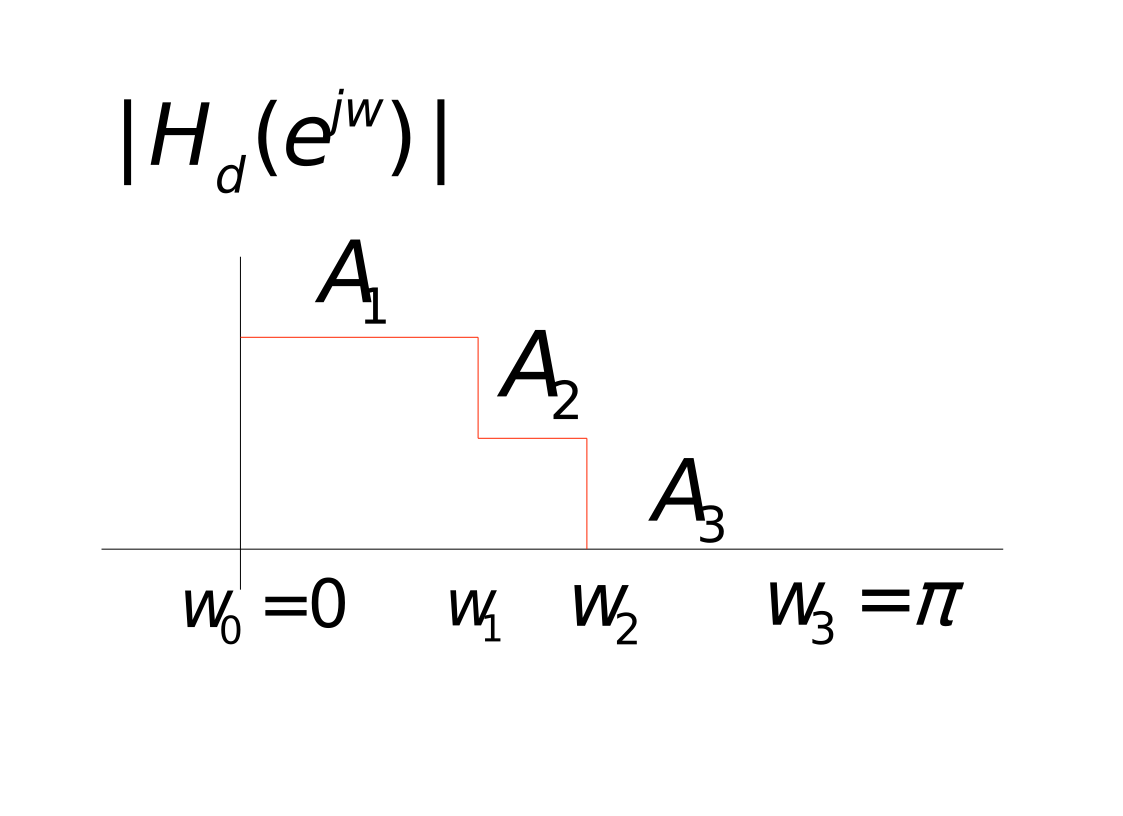
\includegraphics[trim=0cm 1cm 0cm 1cm,clip=true,width=3.5cm]{Figures/PorTramos}


$\scriptsize H_{MNd}(e^{jw})\!=A_k,  \:\:\: w_{k-1}\le|w|\le w_k$

\hspace{1.4cm}$k\!\in\![0,M]$

\hspace{1.0cm}$w_0\!=\!0$

\hspace{1.1cm}$w_M\!=\!\pi$


\vspace{0.1cm}
\color{gray}


\vspace{0.1cm}

$H_{MNd}(e^{jw})=\sum_{k=1}^{M}A_{k}H_{BPd,[w_{k-1},w_k]}(e^{jw})$


\vspace{0.1cm}

\color{black}

$h_{MNd}(n)=\!\left \{\!\!\!\begin{array}{l}\sum_{k=1}^MA_k\frac{w_k-w_{k-1}}{\pi}, \:\:\:  \:\:\: \:\:\: n=0\\ \sum_{k=1}^M(A_k-A_{k-1})\frac{sen(w_kn)}{\pi n},  \: c.c.\end{array}  \right . $


\vspace{0.1cm}
}

\end{column}
\end{columns}

\end{frame}

\begin{frame}
\frametitle{Diseño del filtro FIR por truncamiento I}

\footnotesize

\begin{itemize}
\item EL filtro FIR correspondiente se puede diseñar truncando la función $h_d(n)$ correspondiente, haciéndola  cero para valores $|n|>L$ y retardándola L unidades temporales.


\visible<2->{
\item A continuación vemos la respuesta en frecuencia de los filtros así obtenidos para diferentes valores de N:

\vspace{-0.4cm}



\begin{columns}[c]
\begin{column}{5cm}
\lstinputlisting{./Matlab/FIRLowTrunc.m}


 \end{column}
\hspace{-0.5cm} \begin{column}{5cm}

\centering

\visible<3->{

\scriptsize
Filtro paso bajo



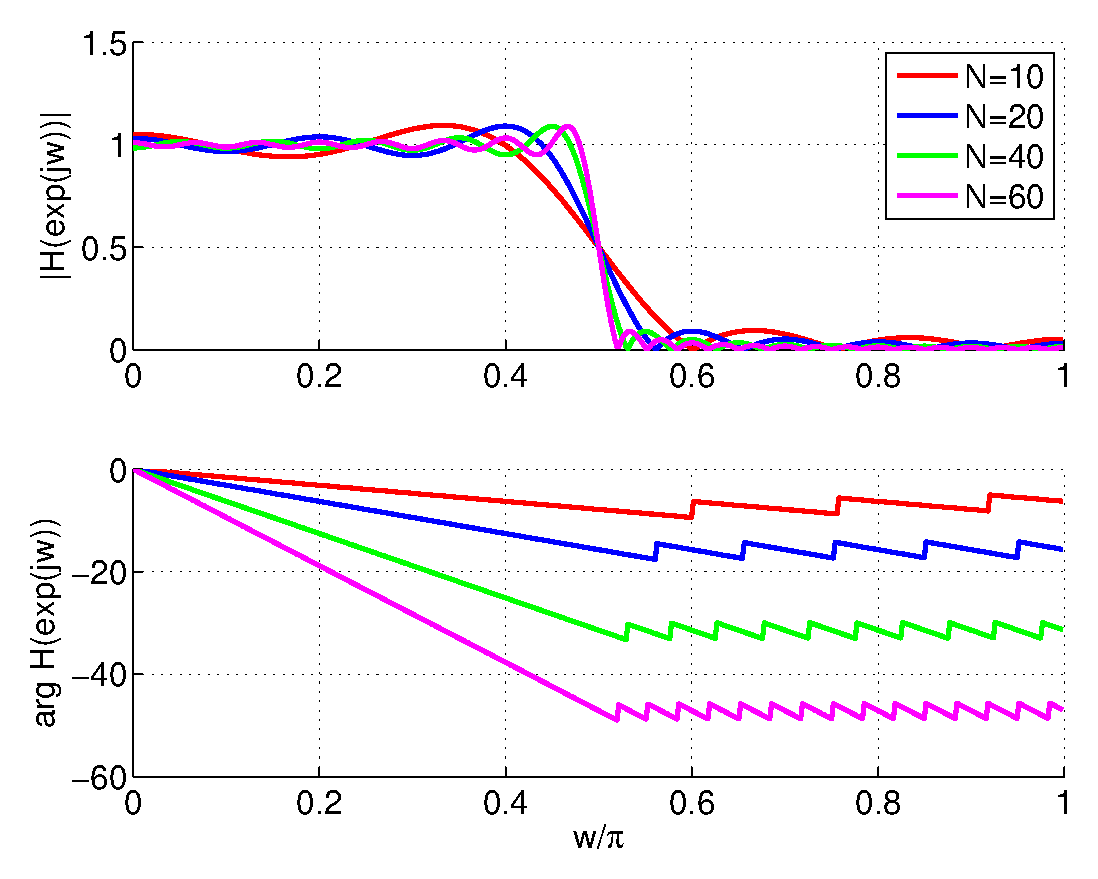
\includegraphics[width=5cm]{Figures/FIRLowTrunc.eps}
}

\visible<4->{
Desfase lineal ($-wN/2$, discont. $\pi$)

$N$ crece $\rightarrow \#_{rizos}$ crece

Tamaño rizos es constante.
}
 \end{column}
 \end{columns}
}


\end{itemize}

\end{frame}

%%%%%%%%%%%%%%%%%%%%%%%%%%

\begin{frame}
\frametitle{Diseño del filtro FIR por truncamiento II}

\begin{columns}[c]
\begin{column}{5cm}
\centering
\scriptsize

Filtro paso bajo

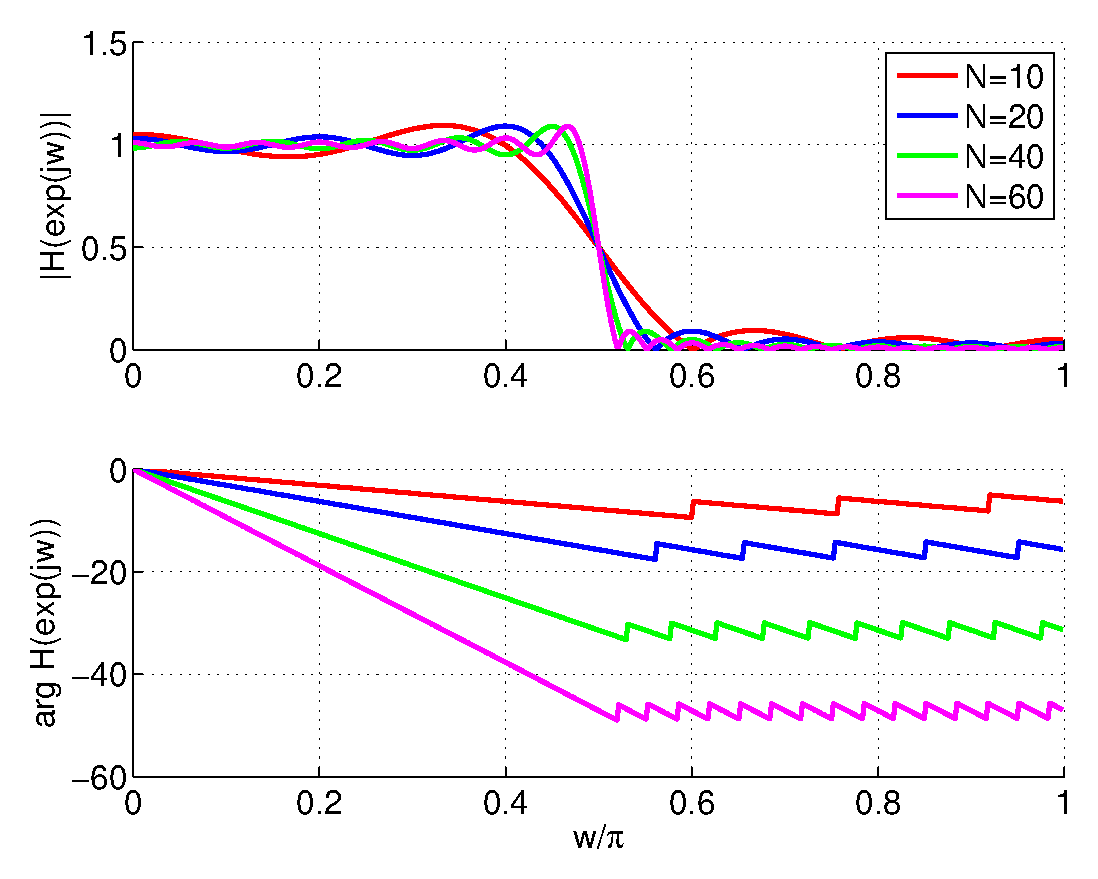
\includegraphics[width=4cm]{Figures/FIRLowTrunc.eps}

\visible<2->{

Filtro paso alto

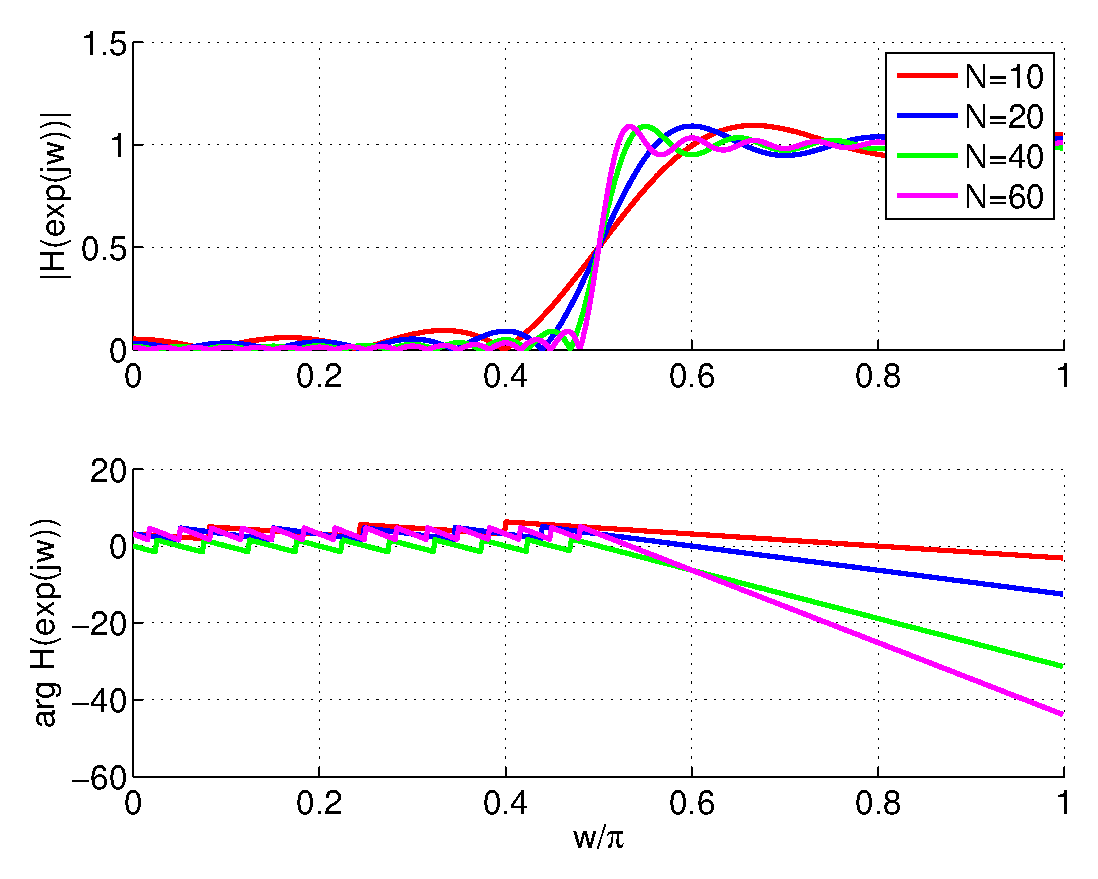
\includegraphics[width=4cm]{Figures/FIRHighTrunc.eps}

}

 \end{column}
\hspace{-0.5cm} \begin{column}{5cm}
\scriptsize

\visible<3->{
Filtro paso banda
\centering

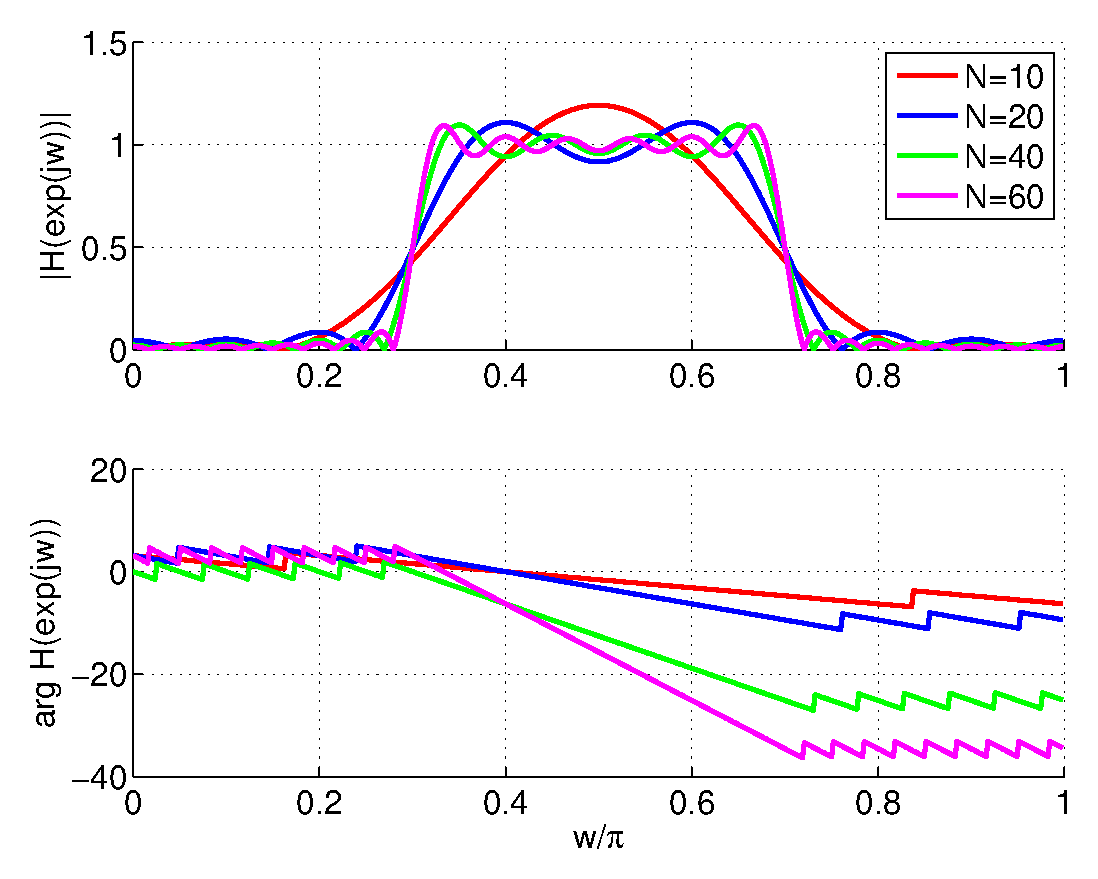
\includegraphics[width=4cm]{Figures/FIRPassTrunc.eps}

Filtro supresor banda

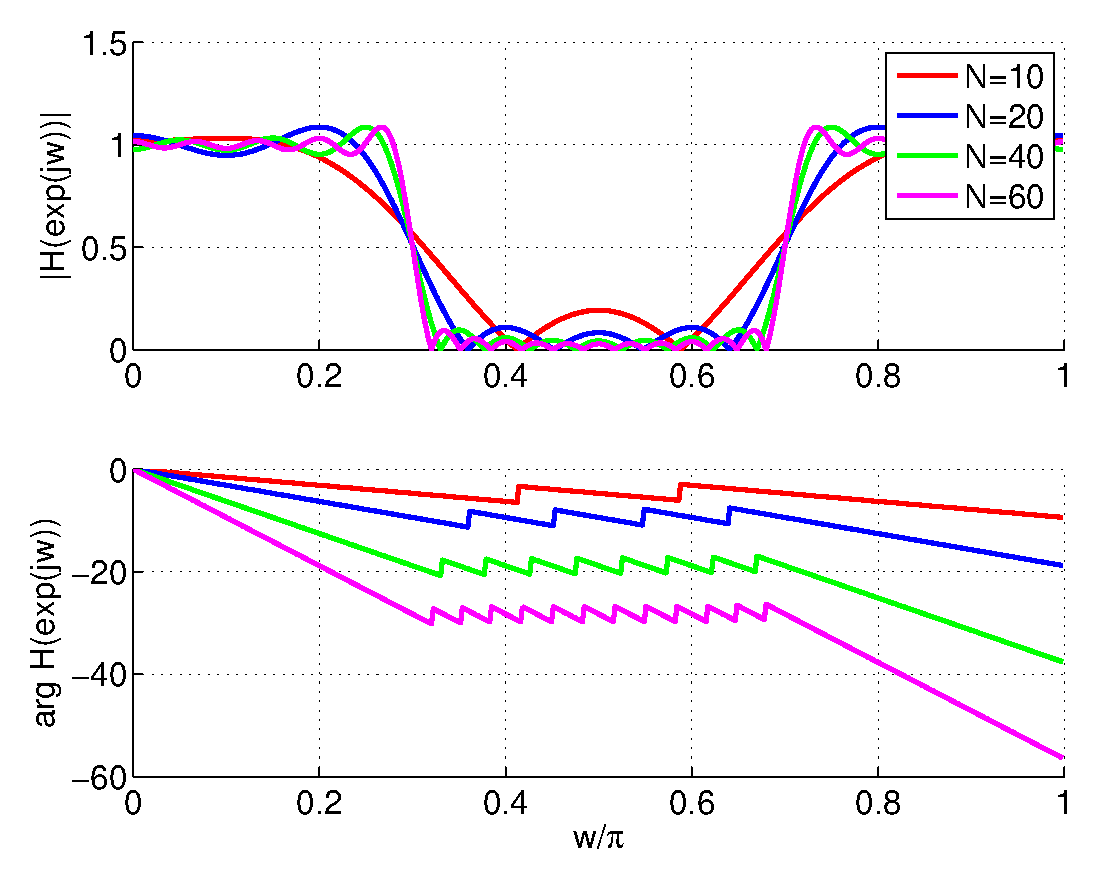
\includegraphics[width=4cm]{Figures/FIRStopTrunc.eps}

}

 \end{column}
 \end{columns}

\scriptsize

{

Desfase lineal ($-wN/2$, discont. $\pi$); tamaño rizos en el borde es constante; y según $N$ crece $\rightarrow \#_{rizos}$ crece, los rizos son más estrechos y la banda de transición decrece.
}

\end{frame}

%%%%%%%%%%%%%%%%%%%%%%%%%

\begin{frame}
\frametitle{Diseño del filtro FIR por truncamiento III}

\footnotesize

\vspace{-0.3cm}

\begin{itemize}
\item Los rizos que se producen tanto en la banda de paso como en la banda de supresión al truncar el filtro son una consecuencia directa del proceso de truncamiento. Este hecho se llama  fenómeno de Gibbs.

\visible<2->{

\item El truncamiento se puede expresar  alternativamente como el producto de la $h_d(n)$ y una ventana $v(n)$ cuadrada de longitud 2L+1: $h_t(n)\!\!=\!\!v(n)h_d(n)$.
}

\visible<3->{
\item Propiedad producto: $h_t(n)=v(n)h_d(n)$} \visible<4->{$\leftrightarrow H_t(e^{jw})=\frac{1}{2\pi}(V*H_d)_{2\pi}(e^{jw})$
}

\visible<5->{
$H_t(e^{jw})=\frac{1}{2\pi}\int_{-\pi}^\pi H_d(e^{jw})V(e^{j(w-\phi)}d\phi$
}
\vspace{-1cm}

\hspace{0.3cm}\begin{columns}[c]
\begin{column}{4cm}
\visible<6->{
$v(n)=\left \{  \begin{array}{l} 1, \:\:-L\le n \le L\\0, \:\: c.c. \end{array} \right .$

\vspace{0.1cm}

$V(e^{jw})=\frac{sen\left([2L+1]w/2\right)}{sen(w/2)}$

\vspace{0.1cm}

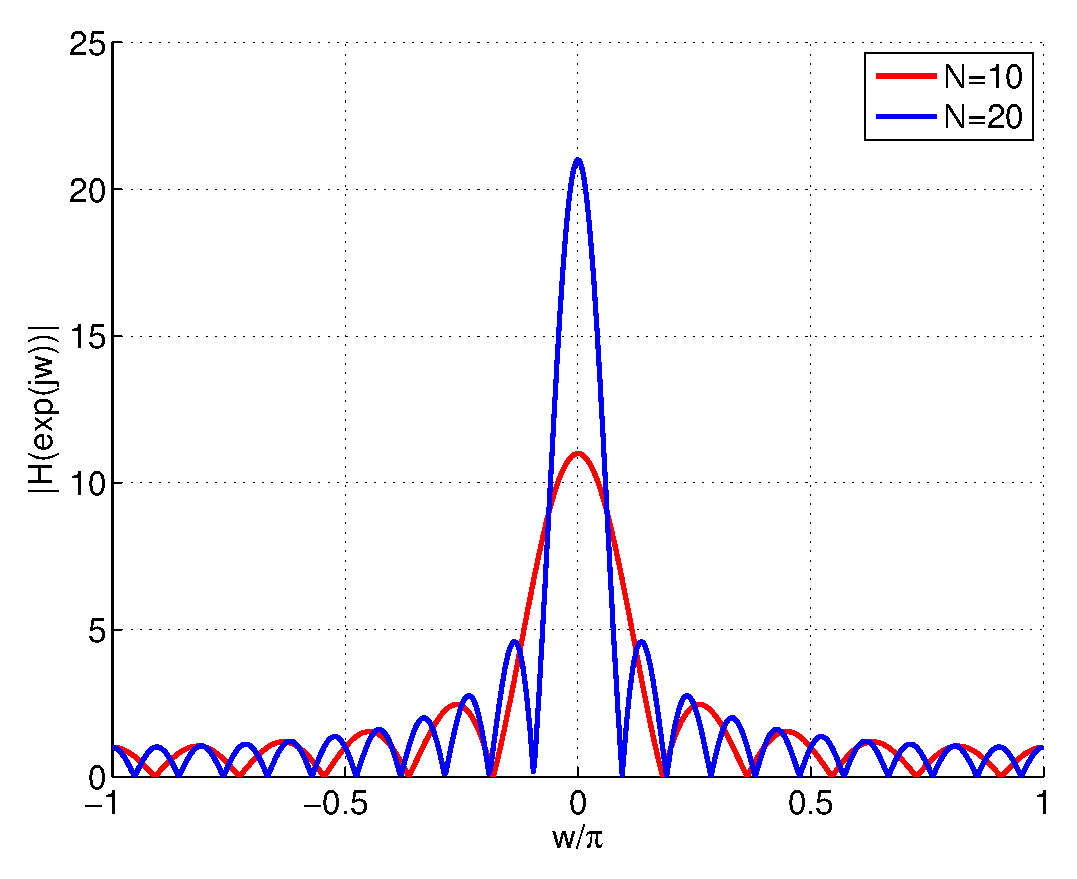
\includegraphics[width=3cm]{Figures/HwTrunc.eps}
}
\end{column}
\hspace{-2cm}\begin{column}{6.5cm}
\visible<7->{
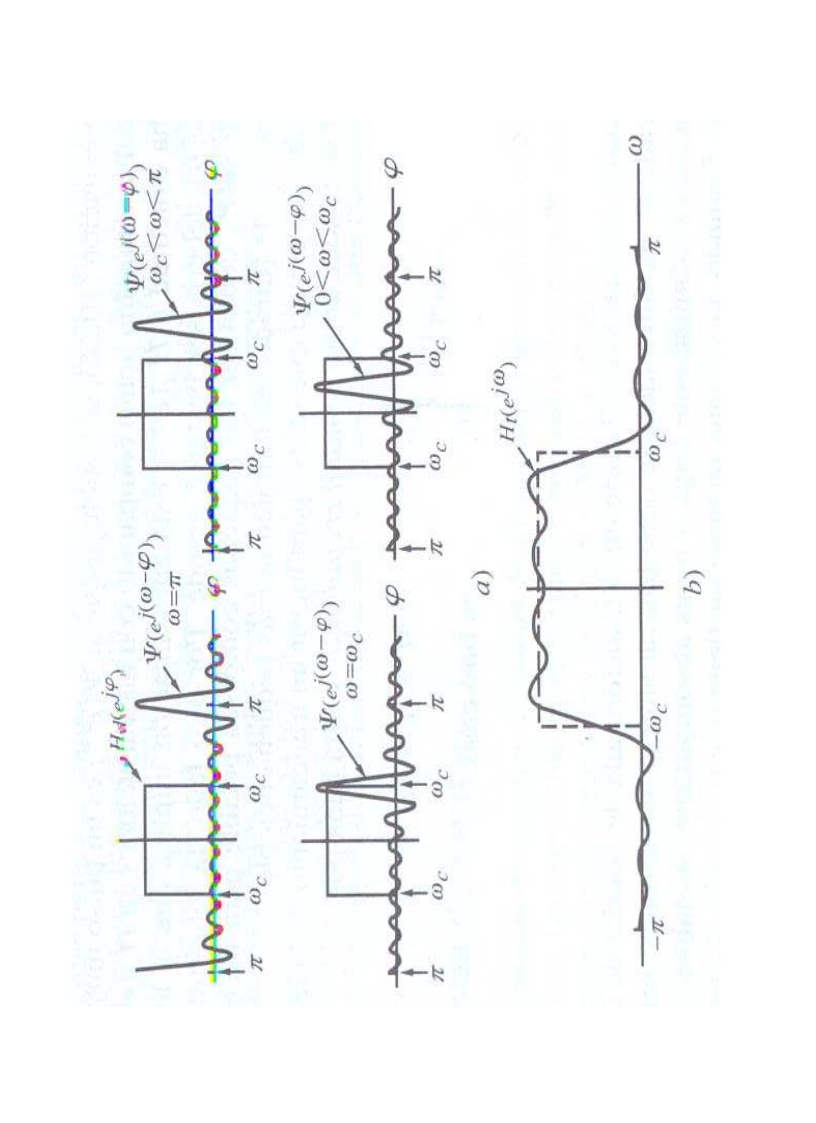
\includegraphics[trim=0cm 1cm 0cm 1cm, clip=true,angle=-90,width=6.5cm]{Figures/ConvTrunc}
}
\end{column}

\end{columns}
\visible<6->{
\vspace{-0.6cm}
\item Si $N$ crece, el lóbulo principal de $V(e^{jw})$ es más estrecho pero el area permanece cte} \visible<7->{ $\rightarrow$ los rizos de $H_t(e^{jw})$ están más cerca de la $w_c$ pero su tamaño permanece cte.
}


\end{itemize}

\end{frame}


%%%%%%%%%%%%%%%%%%%%%%%%%%



\begin{frame}
\frametitle{Diseño del filtro FIR con ventana fija I}

\vspace{-0.4cm}

\footnotesize
\begin{itemize}
\item La aparición del fenómeno de Gibbs se debe a que la ventana $v(n)$ rectangular tiene una transición abrupta.

\visible<2->{
\item Para mitigarlo, se pueden escoger ventanas con transiciones mas suaves ($-L\le n \le L$)
\begin{itemize}
\footnotesize
\item Barlett: $v(n)=1-\frac{|n|}{L+1}$
\item Hann: $v(n)=\frac{1}{2}\left [1+cos\left (\frac{2\pi n}{2L+1}\right )\right ]$
\item Hamming: $v(n)=0.54+0.46 cos \left (\frac{2\pi n}{2L+1}\right )$
\item Blackman: $v(n)=0.42+0.5 cos \left (\frac{2\pi n}{2L+1}\right )+0.08 cos \left (\frac{4\pi n}{2L+1}\right )$
\end{itemize}}
\visible<3->{
\item Las ventanas se pueden obtener con Matlab con las ordenes: \alert{\texttt{rectwin, bartlett, hann, hamming, blackman}.}
\begin{itemize}
\footnotesize
\item Ejemplo: \color{gray} \texttt{v=rectwin(2*L+1)}\color{black}
\end{itemize}}
\end{itemize}

\vspace{-0.2cm}

\begin{columns}[c]
\visible<4->{
\hspace{1cm}\begin{column}{4cm}
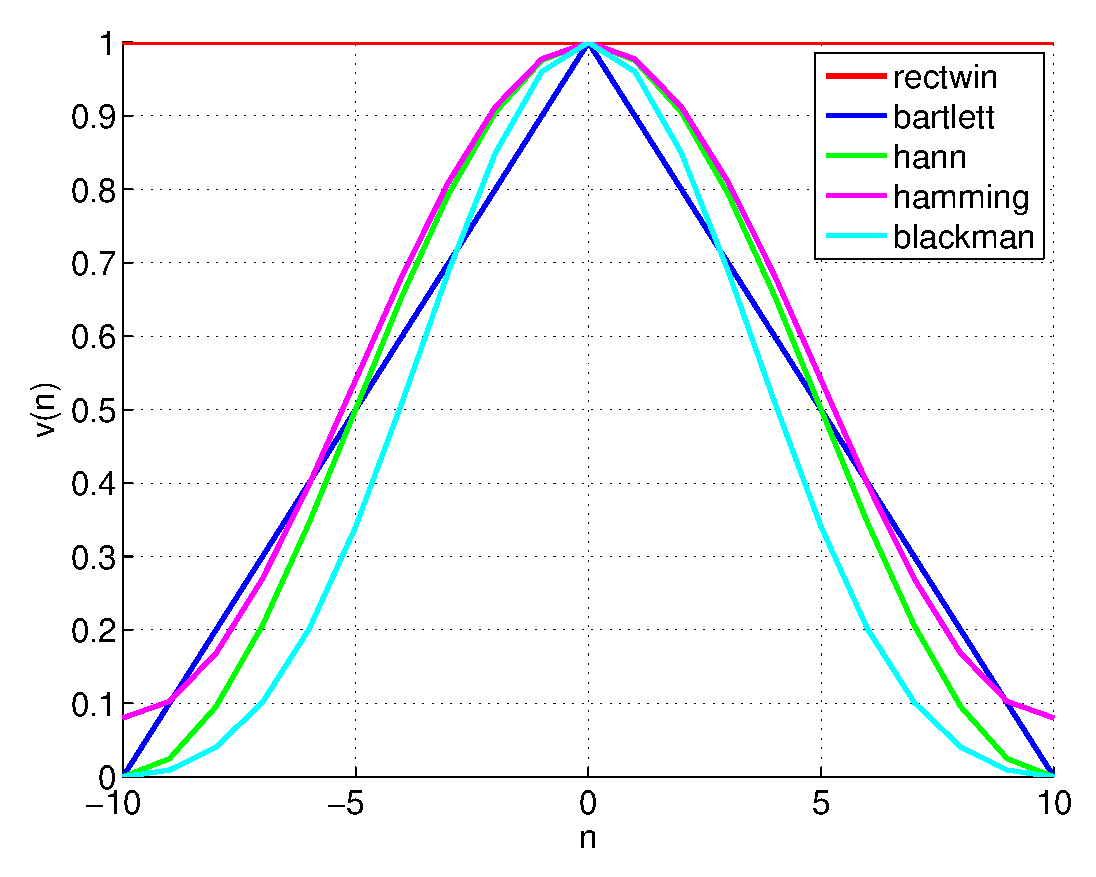
\includegraphics[trim=0cm 0cm 0cm 0cm, clip=true,angle=0,width=3.5cm]{Figures/hnWindow.eps}
\end{column}}

\visible<5->{
\hspace{-0.3cm}\begin{column}{4cm}
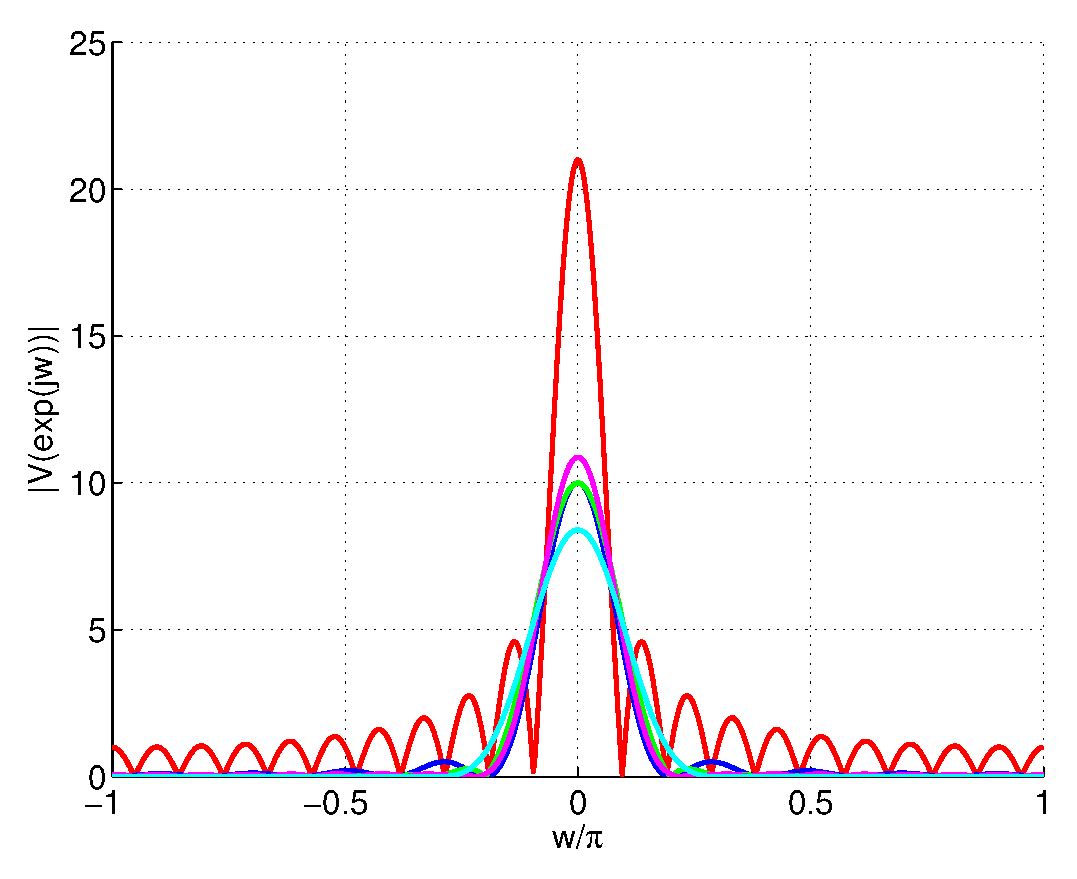
\includegraphics[trim=0cm 0cm 0cm 0cm, clip=true,angle=0,width=3.5cm]{Figures/HwWindow.eps}
\end{column}}
\hspace{-0.2cm}\begin{column}{4cm}
\scriptsize
\visible<5->{
$\Delta_{ML}$: Ancho (frecuencias) del lóbulo principal

$A_{ML}$: Nivel relativo (respecto al siguiente lóbulo) del lóbulo principal

Ambos parámetros están relacionados con el comportamiento de $H_t(n)$
}
\end{column}
\end{columns}

\end{frame}

%%%%%%%%%%%%%%%%%%%%%%%%%%%%%

\begin{frame}
\frametitle{Diseño del filtro FIR con ventana fija II}

\begin{columns}[c]
\begin{column}{7.5cm}
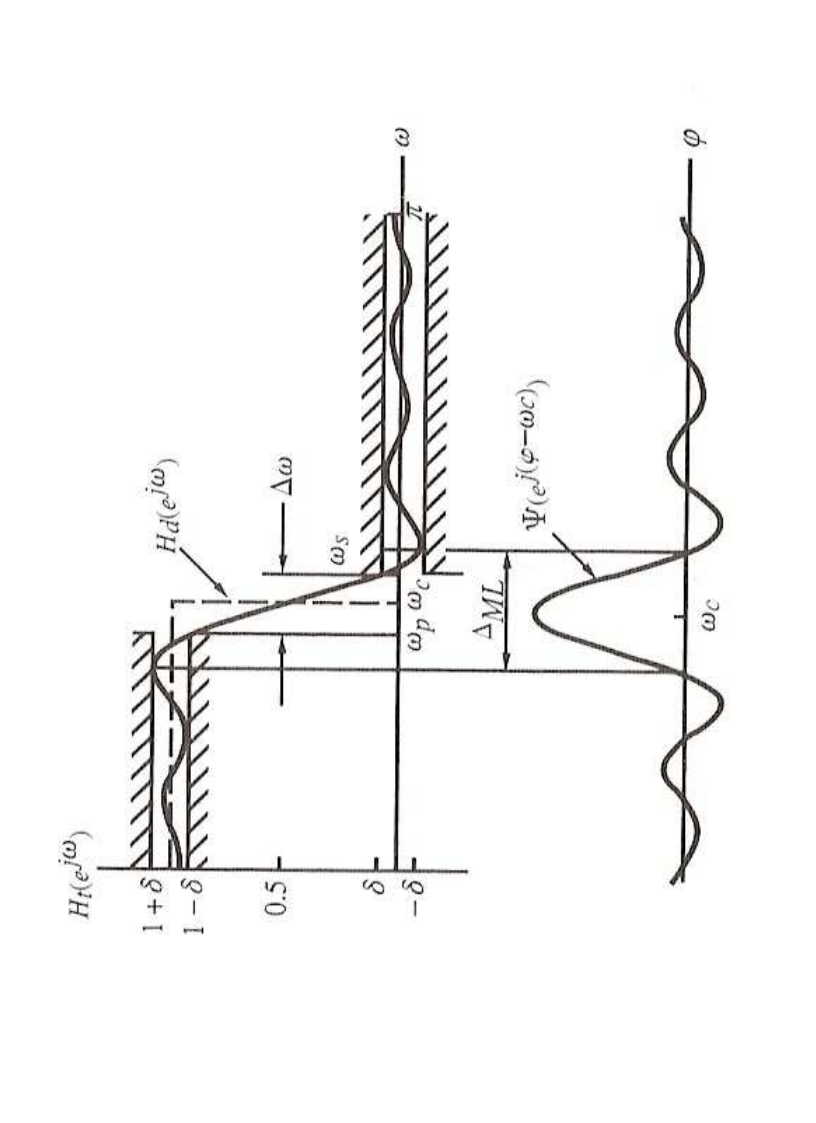
\includegraphics[trim=0cm 0cm 0cm 0cm, clip=true,angle=-90,width=7.5cm]{Figures/WindowFija1}
\end{column}

\hspace{-0.3cm}\begin{column}{4.5cm}

\begin{itemize}
\footnotesize
\item $|H(e^{jw_c})|=0.5$

\item $w_c=\frac{w_p+w_s}{2}$

\item $\Delta_w=w_s-w_p<\Delta_{ML}$

\item Tamaño del rizado $\delta$ es el mismo en ambas bandas

\item Son filtros de ventana fija, porque la atenuación (rizado) es constante.

\visible<2->{
\item M en la tabla es L.}
\end{itemize}
\end{column}

\end{columns}

\vspace{-0.5cm}
\visible<2->{
\hspace{-0.3cm}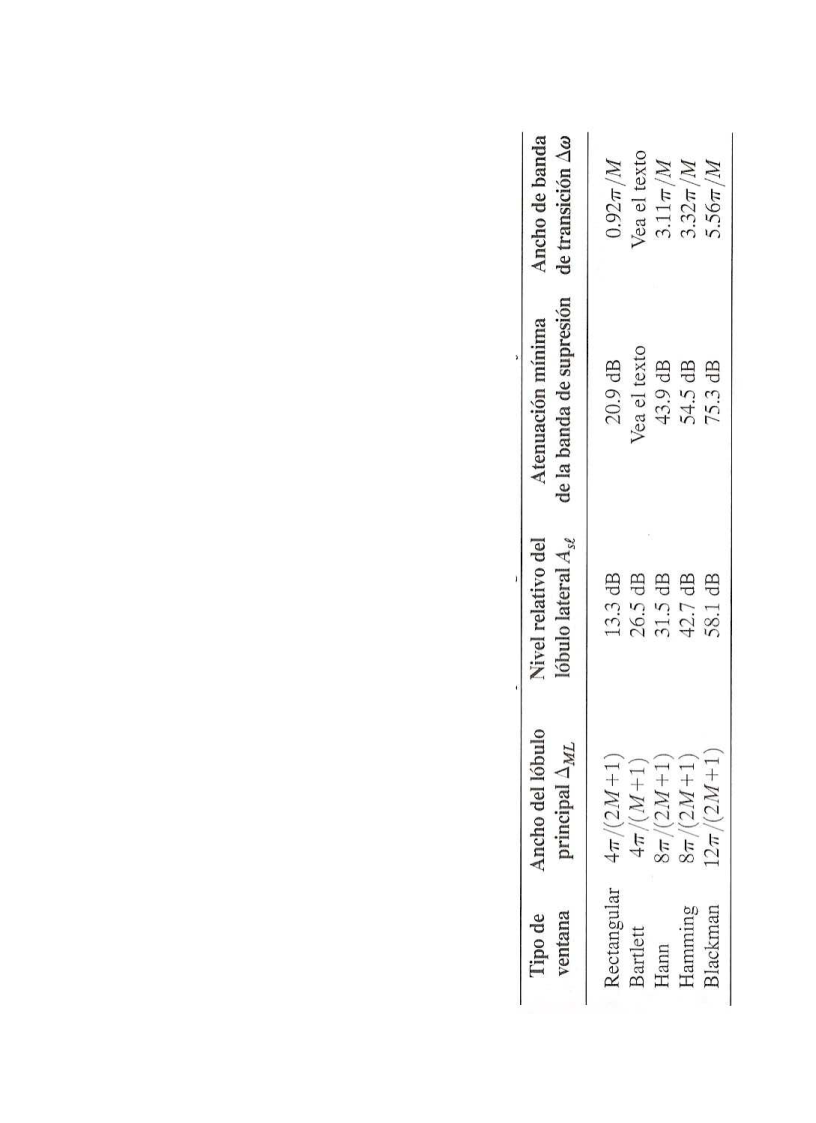
\includegraphics[trim=13cm 0cm 0cm 0cm, clip=true,angle=-90,width=12cm]{Figures/WindowFija2}}

\end{frame}

%%%%%%%%%%%%%%%%%%%%%%%%%%%%%%%%%%%%%%%%%%


\begin{frame}
\frametitle{Ejemplo FIR paso baja de ventana fija}

\footnotesize

\color{olivegreen}Diseñar un filtro paso bajo con las siguientes especificaciones:

 $w_p=0.3\pi$, $w_s=0.5\pi$, $\alpha_s=40dB$.

\color{gray}

\vspace{-0.3cm}

\hspace{-0.3cm}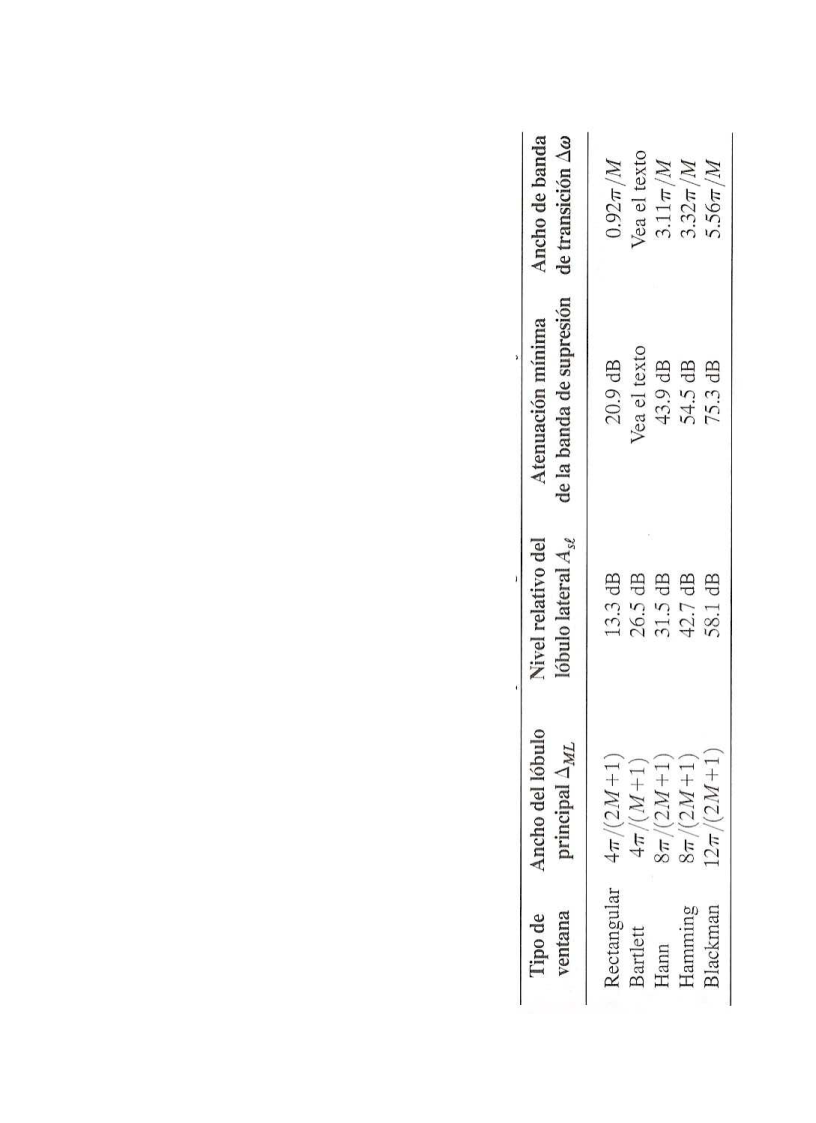
\includegraphics[trim=13.5cm 0cm 1cm 0cm, clip=true,angle=-90,width=10.5cm]{Figures/WindowFija2}

\vspace{-0.1cm}

\scriptsize

 $w_c= \frac{w_p+w_s}{2}=0.4\pi$   $\:\:\:\:\:\Delta_w=w_s-w_p=0.2\pi$

$\alpha_s=40dB$: Filtros posibles son Hann, Hamming, y Hamming



Hann: $\Delta_w=3.11\pi/L  \rightarrow L=3.11\pi/\Delta_w=15.55 \rightarrow L=16$

Hamming: $\Delta_w=3.32\pi/L  \rightarrow L=3.32\pi/\Delta_w=16.6 \rightarrow L=17$

Blackman: $\Delta_w=5.56\pi/L  \rightarrow L=5.56\pi/\Delta_w=27.8 \rightarrow L=28$

\vspace{-0.4cm}

\begin{columns}[T]
\hspace{1cm}\begin{column}{5.5cm}
\lstinputlisting{./Matlab/FIREjemplo1.m}
\end{column}
\hspace{1cm}\begin{column}{4.5cm}

\vspace{0.4cm}
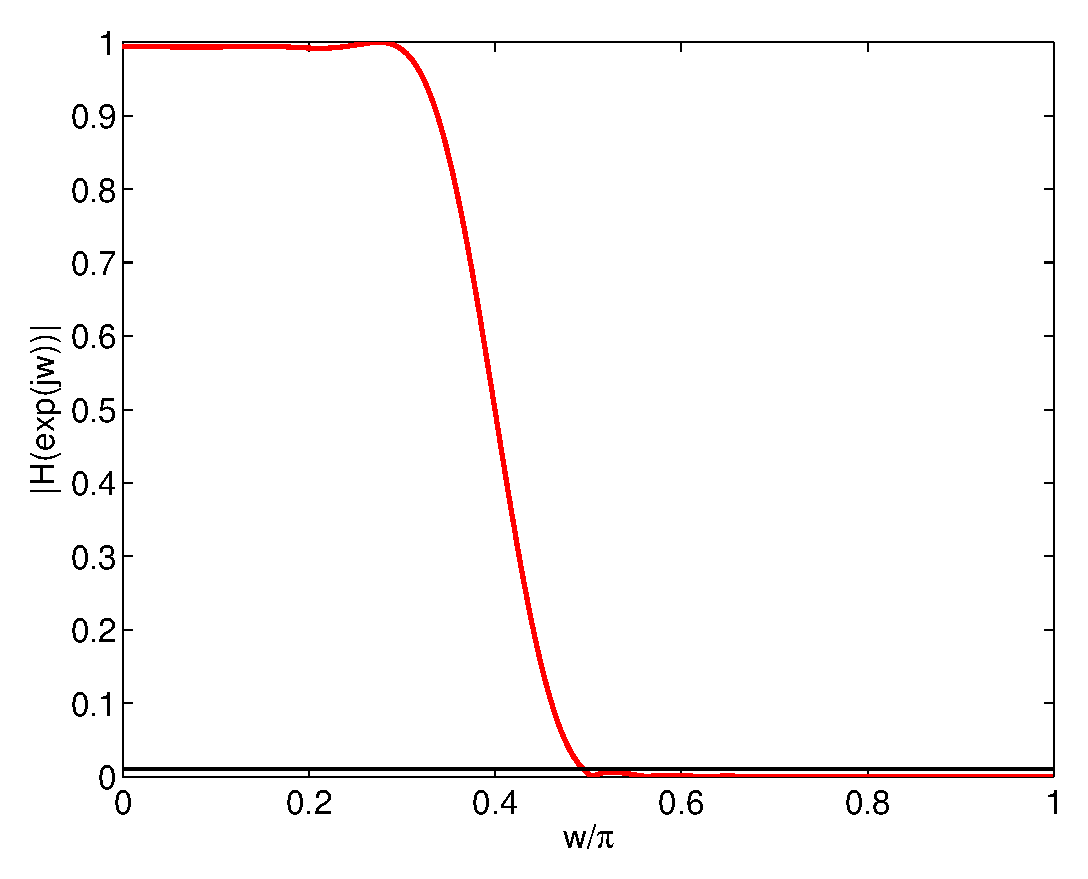
\includegraphics[trim=0cm 0cm 0cm 0cm, clip=true,angle=0,width=4cm]{Figures/FIREx1.eps}

\end{column}
\end{columns}

\end{frame}


%%%%%%%%%%%%%%%%%%%%%%%%%%%%%%%%%
\begin{frame}
\frametitle{Diseño del filtro FIR con ventana variable}
\footnotesize
\begin{itemize}
\item  El rizado de las ventanas fijas es constante
\item Para tener control sobre el valor del rizado, se  pueden usar las ventanas ajustables:
\begin{itemize}
\footnotesize
\item \alert{Dolph-Chebyshev}: \texttt{ v=chebwin(2*L+1,Asl)}
$v(n)=\frac{1}{2L+1}\left[ \frac{1}{\gamma}+\sum_{k=1}^L T_{2N}\left( \beta cos (\frac{k\pi}{2L+1})\right) cos (\frac{2nk\pi}{2L+1})\right]$

$\gamma=\frac{\mathrm{amplitud \:\: lobulo  \:\: lateral}}{\mathrm{amplitud \:\: lobulo  \:\: principal}}$,  $\:\:\:\beta=cosh\left(\frac{1}{2L}acosh(1/\gamma)\right)$

$T_l(x)=\left \{ \begin{array}{l}cos(l \cdot acos(x)), \:\: |x|<1\\cosh(l \cdot acosh(x)), \:\: |x|<1 \end{array}\right .$
 \alert{$\:\:2L=\frac{2.056\alpha_s-16.4}{2.285\Delta w}$}


\vspace{0.2cm}


\item \alert{Kaiser}: \texttt{ v=kaiser(2*L+1,beta)}

\vspace{0.1cm}

$v(n)=\frac{I_o\left(\beta \sqrt{1-(n/L)^2}\right)}{I_o\left(\beta\right)}$

\vspace{0.1cm}

$I_o(u)=1+\sum_{r=1}^\infty \left(\frac{(u/2)^r}{r!}\right).$

$\beta=\left\{\begin{array}{l}0.11102(\alpha_s-8.7), \:\: \alpha_s>50\\0.5482(\alpha_s-21)^{0.4}+0.07886(\alpha_s-21), \:\: 50 \le \alpha_s \le 21\\0, c.c.\end{array} \right .$


\alert{$2L=\frac{\alpha_s-8}{2.285\Delta w}$}

\end{itemize}

\end{itemize}

\end{frame}

%%%%%%%%%%%%%%%%%%%%%%%%%%%%%%%%

\begin{frame}
\frametitle{Ejemplo FIR paso baja de ventana Dolph-Chebyshev}

\footnotesize

\color{olivegreen}Diseñar un filtro paso bajo con las siguientes especificaciones:

 $w_p=0.3\pi$, $w_s=0.5\pi$, $\alpha_s=40dB$.

\color{gray}

 $w_c= \frac{w_p+w_s}{2}=0.4\pi$   $\:\:\:\:\:\Delta_w=w_s-w_p=0.2\pi$

$2L=\frac{2.056\alpha_s-16.4}{2.285\Delta w}  \rightarrow L=22.92  \rightarrow L=23$


\begin{columns}[T]
\hspace{1cm}\begin{column}{5.5cm}
\lstinputlisting{./Matlab/FIREjemplo2.m}
\end{column}
\hspace{1cm}\begin{column}{4.5cm}

\vspace{0.4cm}
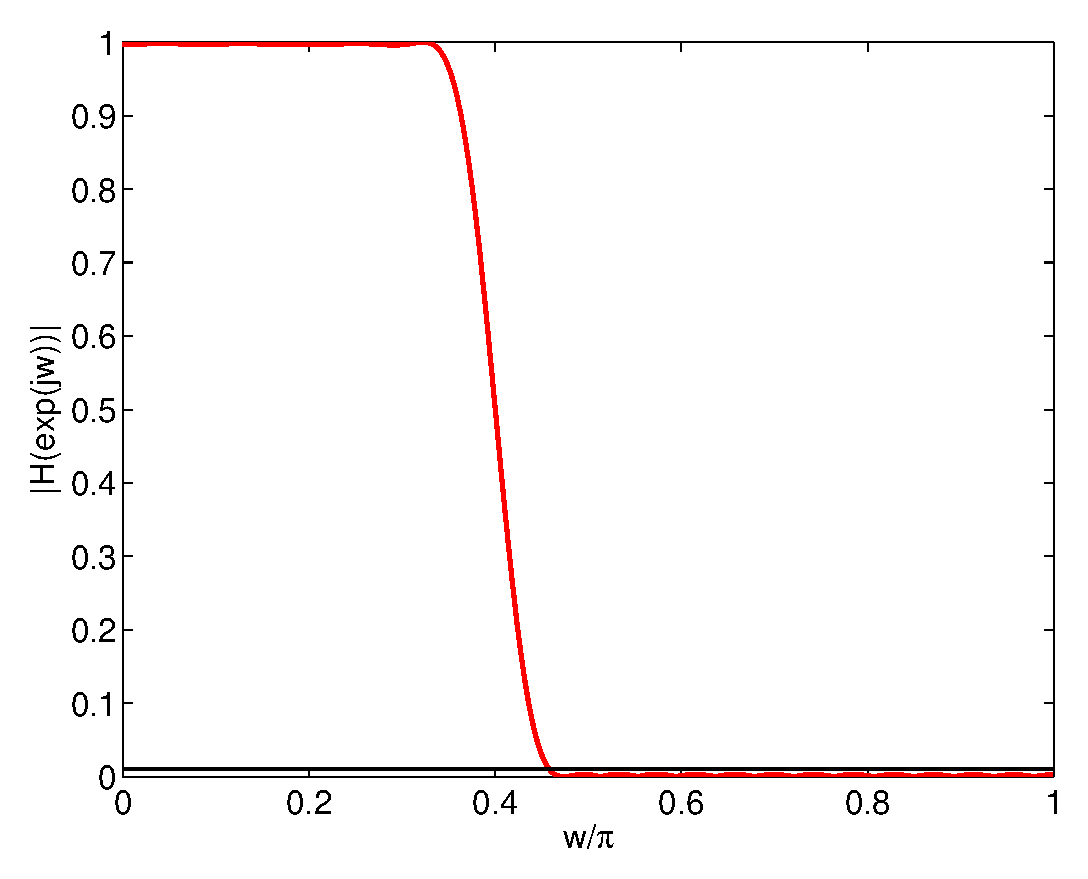
\includegraphics[trim=0cm 0cm 0cm 0cm, clip=true,angle=0,width=4.2cm]{Figures/FIREx2.eps}

\end{column}
\end{columns}

\end{frame}


\begin{frame}
\frametitle{Ejemplo FIR paso baja de ventana Kaiser}

\footnotesize

\color{olivegreen}Diseñar un filtro paso bajo con las siguientes especificaciones:

 $w_p=0.3\pi$, $w_s=0.5\pi$, $\alpha_s=40dB$.

\color{gray}

 $w_c= \frac{w_p+w_s}{2}=0.4\pi$   $\:\:\:\:\:\Delta_w=w_s-w_p=0.2\pi$

$2L=\frac{\alpha_s-8}{2.285\Delta w}  \rightarrow L=11.14  \rightarrow L=12$

$\beta=0.5482(\alpha_s-21)^{0.4}+0.07886(\alpha_s-21)=3.2784$

\begin{columns}[T]
\hspace{1cm}\begin{column}{5.5cm}
\lstinputlisting{./Matlab/FIREjemplo3.m}
\end{column}
\hspace{1cm}\begin{column}{4.5cm}

\vspace{0.4cm}
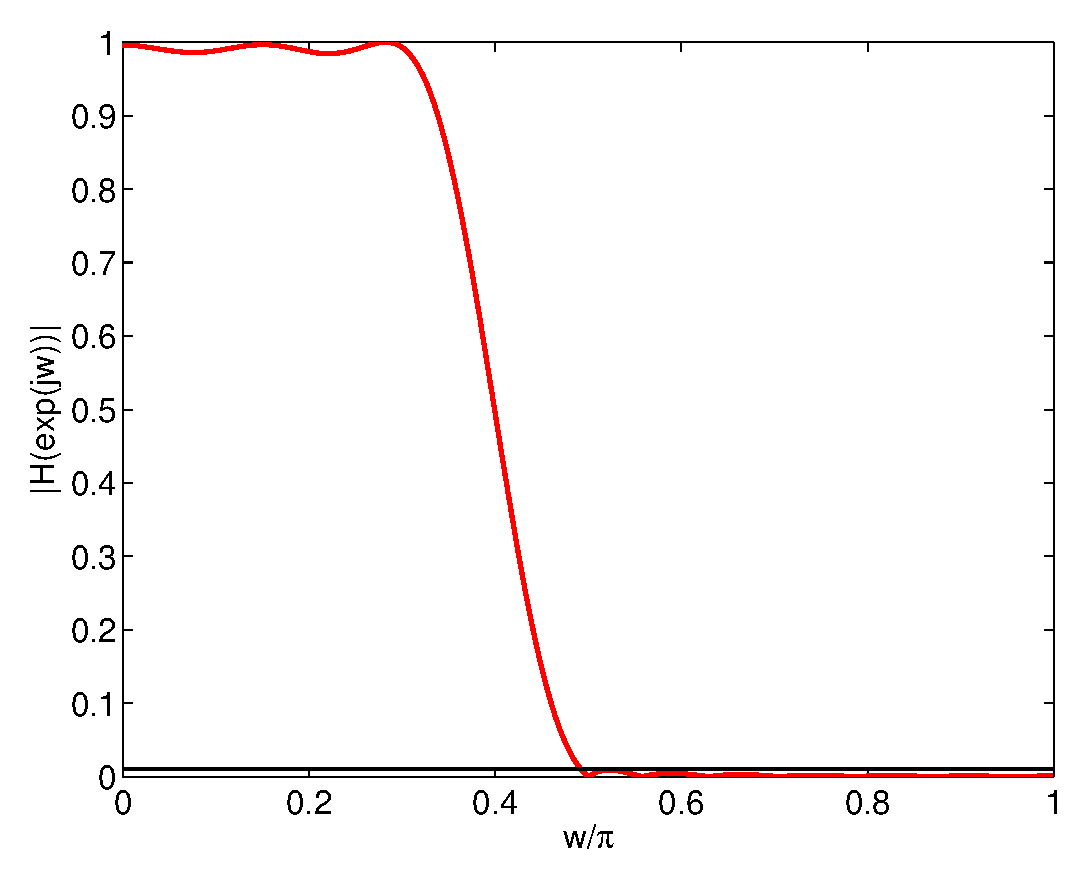
\includegraphics[trim=0cm 0cm 0cm 0cm, clip=true,angle=0,width=4.2cm]{Figures/FIREx3.eps}

\end{column}
\end{columns}

\end{frame}

%%%%%%%%%%%%%%%%%%%%%%%

\begin{frame}
\frametitle{Diseño de filtros avanzados con Matlab}
\footnotesize
\begin{itemize}
\item Adicionalmente, Matlab facilita los cálculos con ordenes adicionales:
\begin{itemize}
\footnotesize
\item Ordenes relacionadas con la ventana de Kaiser:

\texttt{[N,wc,beta,type]=kaiserord([wp,ws],[A1,A2],[dp,ds])}

\texttt{window=kaiser(N+1,beta);}

\texttt{h=fir1(N,wc,type,window);}

\item Ordenes para el diseño de filtros  multinivel:


\texttt{ws=[w0,w1,...,wM];}

\texttt{A=[A0,A1,...AM];}

\texttt{h=fir2(N,ws,A,window)};



\end{itemize}
\end{itemize}
\end{frame}




\begin{frame}
\frametitle{Ejemplo FIR paso alto de ventana Kaiser}

\footnotesize

\color{olivegreen}Diseñar un filtro paso alto con las siguientes especificaciones:

 $w_p=0.55\pi$, $w_s=0.4\pi$, $\delta_s=0.01$.

\color{gray}

\begin{columns}[T]
\begin{column}{6.5cm}
\lstinputlisting{./Matlab/FIREjemplo4.m}
\end{column}
\hspace{-0.5cm}\begin{column}{4.5cm}

\vspace{0.4cm}
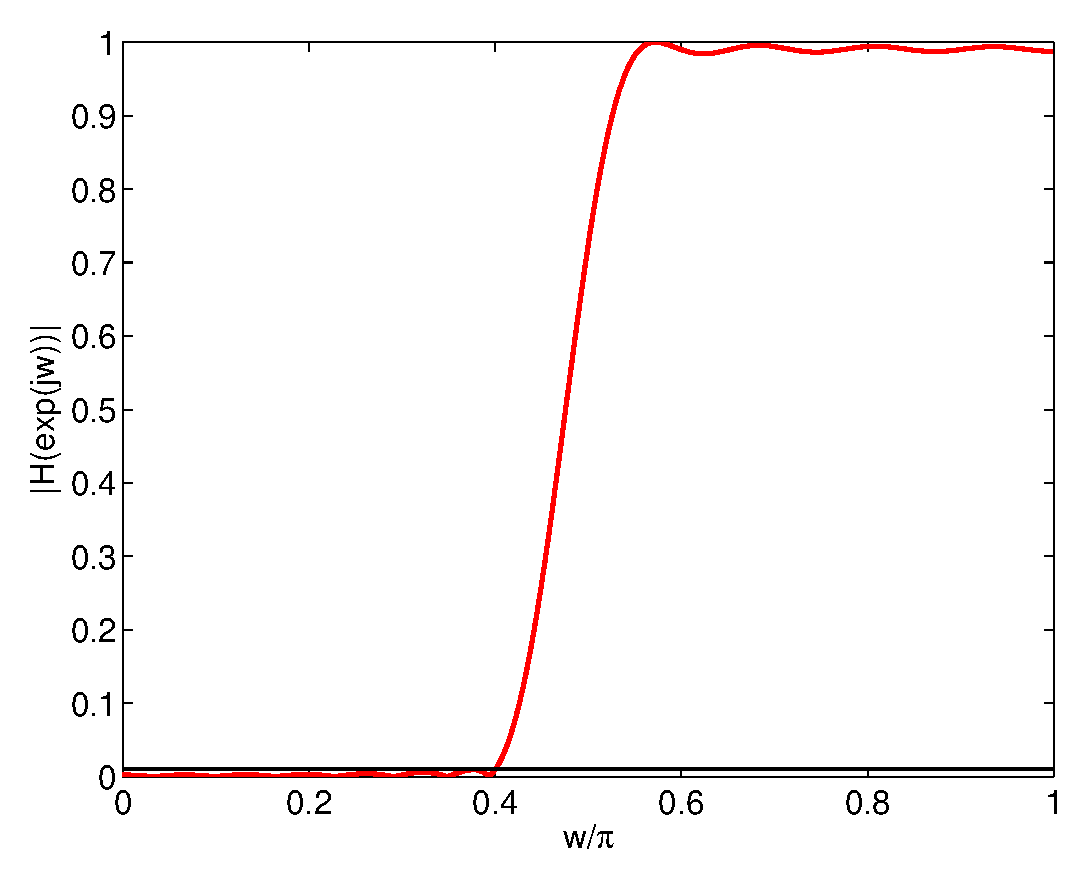
\includegraphics[trim=0cm 0cm 0cm 0cm, clip=true,angle=0,width=4.2cm]{Figures/FIREx4.eps}

\end{column}
\end{columns}

\end{frame}

%%%%%%%%%%%%%%%%%%%%%%%%%%%%%%%%%%%%%%%%%%%%%%%


\begin{frame}
\frametitle{Ejemplo FIR multibanda}

\footnotesize

\color{olivegreen}Diseñar un filtro multibanda con ventana de Hamming con las siguientes especificaciones:

w=[0,0.28,0.3,0.5,0.52,1];

A=[0.3,0.3,1.0,1.0,0.7,0.7];


\color{gray}

\begin{columns}[T]
\begin{column}{6.5cm}
\lstinputlisting{./Matlab/FIREjemplo5.m}
\end{column}
\hspace{-0.5cm}\begin{column}{4.5cm}

\vspace{0.4cm}
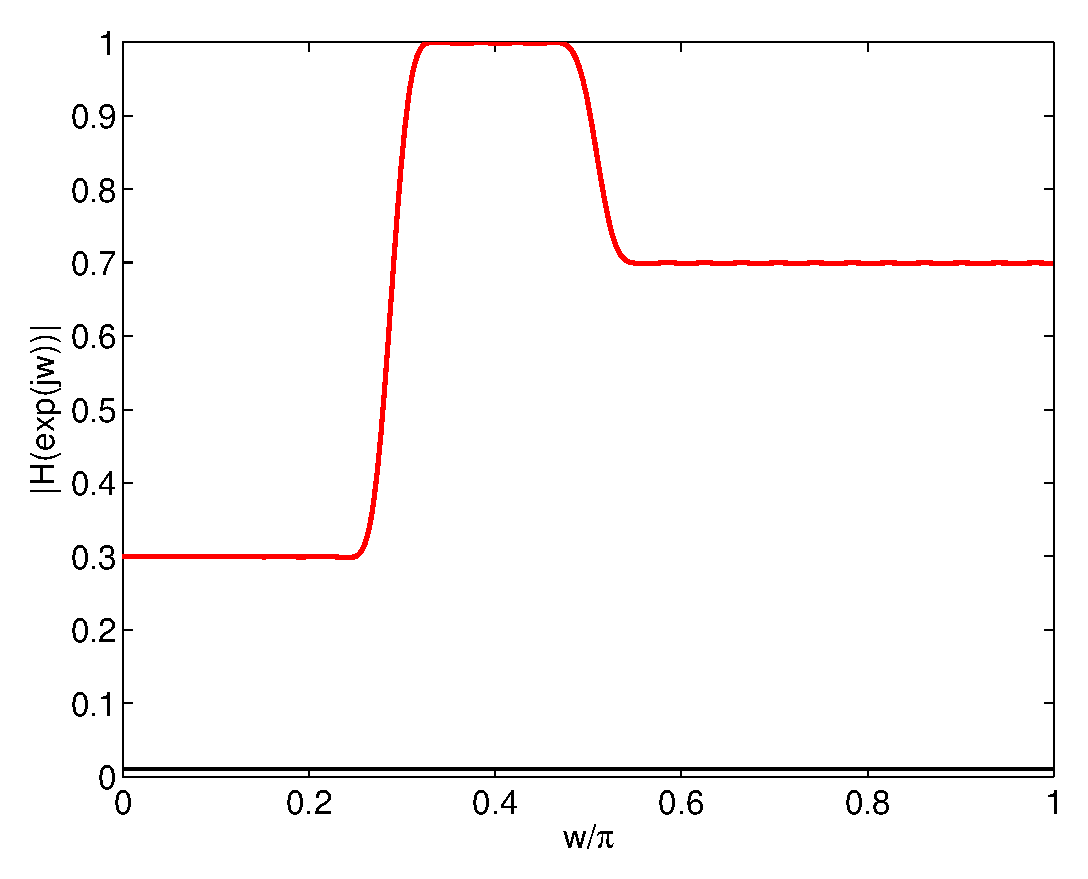
\includegraphics[trim=0cm 0cm 0cm 0cm, clip=true,angle=0,width=4.2cm]{Figures/FIREx5.eps}

\end{column}
\end{columns}

\end{frame}


\begin{frame}
\frametitle{Métodos alternativos cálculo de N}

\vspace{-0.4cm}

\footnotesize
\begin{itemize}
\item Existen expresiones  adicionales para estimar el orden (N+1) del filtro:

\begin{itemize}

\vspace{-0.1cm}

\footnotesize

\item Kaiser: $\displaystyle N \approx \frac{-20 log_{10}\left( \sqrt{\delta_p \delta_s}\right)-13}{14.6(w_s-w_p)/(2\pi)}$

%\vspace{0.1cm}

\item Bellanger: $\displaystyle  N \approx - \frac{-2 log_{10}( 10 \delta_p \delta_s)}{3(w_s-w_p)/(2\pi)}$

%\vspace{0.1cm}

\item Hermann: $\displaystyle  N \approx  \frac{D_\infty(\delta_p,\delta_s)-F_\infty(\delta_p,\delta_s)\left [(w_s-w_p)/(2\pi)\right ]^2}{(w_s-w_p)/(2\pi)}$

{\scriptsize
$D_\infty(\delta_p,\delta_s)=\left [a_1 \left (log_{10}(\delta_p)\right )^2+ a_2 log_{10}(\delta_p)+a_3\right ]log_{10}(\delta_s)-$

\hspace{1.8cm}$-\left [a_4 \left (log_{10}(\delta_p)\right )^2+ a_5 log_{10}(\delta_p)+a_6\right ]$

\vspace{0.1cm}

$F_\infty(\delta_p,\delta_s)=11.01217 + 0.51244 \left ( log_{10}(\delta_p)-log_{10}(\delta_s)\right )$

\vspace{0.1cm}


\hspace{-0.2cm}$\begin{array}{lll}a_1=0.005309 &a_2=0.07114 & a_3=-0.4761 \\ a_4=0.00266 &a_5=0.5941&a_6=0.4278\end{array}$

}


\end{itemize}
\vspace{-0.3cm}
\scriptsize{
\item Si $\delta_p < \delta_s$ hay que cambiar la una por la otra en la fórmula de Hermann
\item Para valores elevados de los rizos es mejor usar la ecuación de Hermann
\item Las formulas estiman N.  Si el filtro no cumple los requisitos, incrementar  N.
\item En los filtros paso/supresor banda, hay dos bandas de transición. Usar la banda más estrecha.}
\end{itemize}

\vspace{-0.4cm}

\rule{12cm}{0.4pt}

\scriptsize

Las formulas están en función de los rizos: $\alpha_p=-20 log_10(1-\delta_p)$, $\alpha_s=-20 log_10(\delta_s)$

\end{frame}


\subsection{Comparativa IIR vs. FIR}

\begin{frame}
\frametitle{Filtros IIR vs. filtros FIR}

{\footnotesize
\hspace{0.5cm}\alert{IIR:} $\displaystyle H(z)=\frac{p_0+p_1 z^{-1}+ \dots +p_M z^{-M}}{d_0+d_1 z^{-1}+ \dots +d_N z^{-N}}$
\hspace{0.5cm}\alert{FIR:} $H(z)=h_0+\dots h_N z^{-N}$}
\begin{itemize}
\small
\item En los filtros FIR solo es posible colocar ceros (atenuar), mientras que en los filtos IIR se puede colocar ceros (atenuar) y polos (amplificar)
\item Para dos filtros del mismo orden N, el número de operaciones de un filtro FIR es menor que el número de operaciones del filtro IIR. 
\item Para dos filtros con las mismas prestaciones (características de la respuesta en frecuencia), el orden del filtro IIR suele ser menor que el orden del filtro FIR
\item Para diseñar filtros de fase (desfase) lineal se puede:
\begin{itemize}
\item Si el filtro es FIR, usar las técnicas de TF con ventana o hacer que las $h(n)$ cumplan una relaciones especiales. 
\item Si el filtro es IIR, introducir un filtro paso todas que modifique el desfase introducido por el filtro IIR. La introducción del filtro paso todas reduce el ahorro computacional debido a la reducción del orden del filtro.
\end{itemize}

\end{itemize}
\end{frame}
